\documentclass{cls/thesis}
% CSS
\lstdefinelanguage{CSS}{
  keywords={color,background-image:,margin,padding,font,weight,display,position,top,left,right,bottom,list,style,border,size,white,space,min,width, transition:, transform:, transition-property, transition-duration, transition-timing-function},	
  sensitive=true,
  morecomment=[l]{//},
  morecomment=[s]{/*}{*/},
  morestring=[b]',
  morestring=[b]",
  alsoletter={:},
  alsodigit={-}
}

% JavaScript
\lstdefinelanguage{JavaScript}{
  morekeywords={typeof, new, true, false, catch, function, return, null, catch, switch, var, let, if, in, while, do, else, case, break},
  morecomment=[s]{/*}{*/},
  morecomment=[l]//,
  morestring=[b]",
  morestring=[b]'
}

\lstdefinelanguage{HTML5}{
  language=html,
  sensitive=true,	
  alsoletter={<>=-},	
  morecomment=[s]{<!-}{-->},
  tag=[s],
  otherkeywords={
  % General
  >,
  % Standard tags
	<!DOCTYPE,
  </html, <html, <head, <title, </title, <style, </style, <link, </head, <meta, />,
	% body
	</body, <body,
	% Divs
	</div, <div, </div>, 
	% Paragraphs
	</p, <p, </p>,
	% scripts
	</script, <script,
  % More tags...
  <canvas, /canvas>, <svg, <rect, <animateTransform, </rect>, </svg>, <video, <source, <iframe, </iframe>, </video>, <image, </image>, <header, </header, <article, </article
  },
  ndkeywords={
  % General
  =,
  % HTML attributes
  charset=, src=, id=, width=, height=, style=, type=, rel=, href=,
  % SVG attributes
  fill=, attributeName=, begin=, dur=, from=, to=, poster=, controls=, x=, y=, repeatCount=, xlink:href=,
  % properties
  margin:, padding:, background-image:, border:, top:, left:, position:, width:, height:, margin-top:, margin-bottom:, font-size:, line-height:,
	% CSS3 properties
  transform:, -moz-transform:, -webkit-transform:,
  animation:, -webkit-animation:,
  transition:,  transition-duration:, transition-property:, transition-timing-function:,
  }
}

\usepackage{listings}
\usepackage{xcolor}
\usepackage{ragged2e} 

% for text alignment
\justifying              % globally justify all text
\setlength{\parindent}{1cm}   % indentation for each new paragraph
\setlength{\parskip}{0pt}
\lstset{
    basicstyle=\ttfamily\footnotesize,   % font for code
    breaklines=true,                      % automatically break long lines
    breakatwhitespace=true,               % break at spaces if needed
    showstringspaces=false,
    numbers=left,
    numberstyle=\tiny\color{gray},
    frame=single,
    keywordstyle=\color{blue},
    commentstyle=\color{green!60!black},
    stringstyle=\color{orange},
    tabsize=2,
    captionpos=b
}





\hyphenpenalty=10000
\begin{document}
\maketitle
\fontsize{12}{12}\selectfont	
\pagestyle{plain}
\begin{spacing}{1.5}
\justifying 
% {
% \thispagestyle{empty}
% \vspace*{0.5cm}
% \fontsize{13}{13}\selectfont
% \centering{\MakeUppercase{\textbf{DEPARTMENT OF COMPUTER APPLICATIONS}}} \\
% \centering{\MakeUppercase{\textbf{GOVERNMENT ENGINEERING COLLEGE, THRISSUR}}} \\
% \centering{\MakeUppercase{THRISSUR, KERALA STATE, PIN 680009 }} \\
% \vspace*{0.5cm}

% \begin{figure}[ht]
% \centering
% 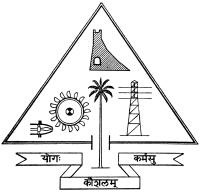
\includegraphics[scale=.8]{image/2.jpg}
% \end{figure}

% \vspace{0.7cm}
% \fontsize{14}{14}\selectfont
% \textbf{\centering CERTIFICATE}\\

% \vspace{0.5cm}
% \fontsize{12}{12}\selectfont
% \noindent
% \textit{This is to certify that the mini project titled } \textbf{\MakeUppercase{"AI Based Form Filling Assistant using Document Intelligence"}} \textit{is a bonafide work done by} \textbf{GOPIKA K (TCR24MCA-2033)} \textit{under my supervision and guidance, and is submitted in October 2025 in partial fulfillment of the requirements for the award of the Degree of Master of Computer Applications from APJ Abdul Kalam Technological University (KTU).}

% \vspace*{2.2cm}

% % \noindent
% % \begin{tabular}{p{5.2cm} p{5.2cm} p{5.2cm}}
% % \centering \textbf{Prof. Soumya Chandran} & \centering \textbf{Prof. Sreejith V.P.} & \centering \textbf{Dr. Sminesh C N} \\
% % \centering Project Guide 
% % \centering Project Coordinator  \\

% \vspace*{2 cm}
% \noindent{
% 	\begin{tabular}{p{4cm}cp{7cm}}
%         Prof.~ ~Soumia~Chandran~M&\hspace{1.5cm}Prof. Sreejith V P&\hspace{1.5cm}Dr. Sminesh C N\\
	      
% 		\textbf{Project Guide} &  \hspace{1.5cm} \textbf{Project Coordinator} &  \hspace{2cm}  \textbf{HOD} \\\\\\
	
% 		Place : THRISSUR & \hfill\\
% 		Date : 10-10-2025  &   \\\\\\
% 	\end{tabular}
% }

% \newpage

\justifying
\thispagestyle{empty}
\vspace*{0.5cm}
\fontsize{13}{13}\selectfont
\centering{\MakeUppercase{\textbf{DEPARTMENT OF COMPUTER APPLICATIONS}}} \\
\centering{\MakeUppercase{\textbf{GOVERNMENT ENGINEERING COLLEGE, THRISSUR}}} \\
\centering{\MakeUppercase{THRISSUR, KERALA STATE, PIN 680009 }} \\
\fontsize{12}{12}\selectfont
\vspace*{0.5cm}
\begin{figure}[ht]
{\centering {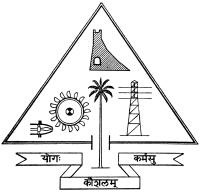
\includegraphics[scale=.8]{image/2.jpg}}\par}
\end{figure}
\vspace{0.7cm}
\fontsize{14}{14}\selectfont
\textbf{\centering{CERTIFICATE}}\\
\justify
\vspace{0.5cm}
\fontsize{12}{12}\selectfont
\textit{This is to certify that the main project titled }
\textbf{\MakeUppercase{``AI-POWERED CODE DOCUMENT GENERATOR"}}
\textit{is a bonafide work done by} \textbf{ARYA K A}  \textbf{(TCR24MCA-2020)}
\textit{under my supervision and guidance, and is submitted in March 2026 in partial fulfillment of the requirements for the award of the Degree of Master of Computer Applications from APJ Abdul Kalam Technological University (KTU).}
\\
\vspace*{2 cm}

\noindent



\hspace*{-0.8cm}
\noindent
\begin{tabular*}{\textwidth}{@{}l@{\extracolsep{\fill}}c@{\extracolsep{\fill}}r@{}}

Prof. Sreejith V P & Prof. Raseek C & Dr. Sminesh C N \\
\textbf{Project Guide} & \textbf{Project Coordinator} & \textbf{HOD} \\[2em]

Place : Thrissur & & \\
Date : 31-03-2026 & & \\

\end{tabular*}

\newpage
\chapter*{DECLARATION}
I hereby declare that the main project named, \textbf{\MakeUppercase{AI-POWERED CODE DOCUMENT GENERATOR}}, is my own work and that, to the best of my knowledge and belief, it contains no material previously published by another person nor material which has been accepted for the award of any other degree or course of the university or any other institute of higher learning, except where due acknowledgment and reference has been made in the text.

\vspace{2cm}

\noindent
\begin{tabular*}{\textwidth}{@{\extracolsep{\fill}} l r}
Place : Thrissur & \textbf{ARYA K A} \\
Date : 31-03-2026 & \textbf{(TCR24MCA-2020)} \\
\end{tabular*}

\newpage
% \chapter*{\rm \large \bf ACKNOWLEDGEMENT}
% \par\hspace{1.5cm}I would like to thank  Department of Computer Application, GEC Thrissur, for giving me this opportunity to pursue this project and successfully complete it.

% \par
% \hspace{1cm}I am highly indebted to our head of the department \textbf{Dr. Sminesh C N}, for his guidance and constant supervision as well as providing necessary information regarding the project and also for his support in completing the project.
% \par
% \hspace{1cm}I express my heart-felt gratitude to my project guide \textbf{Prof. Soumia Chandran}, for her committed guidance, valuable suggestions, constructive
% criticisms and precious time that she invested throughout the work.
% \par

%  \hspace{1cm} I \hspace{0.2cm}express\hspace{0.2cm} my\hspace{0.2cm} heart-felt\hspace{0.2cm} gratitude\hspace{0.2cm} to project coordinator\hspace{0.2cm} \textbf{Prof. Sreejith V P}, for her committed guidance as well as providing necessary information regarding the project, and also for her support in completing the project.

% \par
% \hspace{1cm}I sincerely thank all other faculties of MCA department for guiding me through the processes involved in the project.
% \newpage

\chapter*{\rm \large \bf ACKNOWLEDGEMENT}
\par\hspace{0.5cm}
\begin{justify}

\hspace{0.5cm}I would like to thank  Department of Computer Application, GEC Thrissur, for giving me this opportunity to pursue this project and successfully comple-te it.
\end{justify}

\begin{justify}

\hspace{0.5cm}I am highly indebted to our head of the department \textbf{Dr. Sminesh C N}, for his guidance and constant supervision as well as providing necessary information regarding the project and also for his support in completing the project. 
\end{justify}

\begin{justify}

\hspace{0.5cm}I express my heartfelt gratitude to my project guide \textbf{Prof. Sreejith V P}, for his committed guidance, valuable suggestions, constructive
criticisms and precious time that he invested throughout the work.
\end{justify}

\begin{justify}

\hspace{0.5cm}I express my heartfelt gratitude to project coordinator \textbf{Prof. Raseek C}, for his committed guidance as well as providing necessary information regarding the project, and also for his support in completing the project.
\end{justify}

\begin{justify}
    
\hspace{0.5cm}I sincerely thank all other faculties of MCA department for guiding me through the processes involved in the project.
\end{justify}

\newpage
\chapter*{\rm \large \bf ABSTRACT}
\vspace{3.0mm}
\begin{justify}

\hspace{0.5cm}Maintaining software project documentation accurately and up to date is hard because code changes often, and writing documentation by hand takes a lot of time. Outdated documentation can make code harder to understand, require more effort to keep up to date, and pose challenges for new developers who want to join a project. To solve these problems, this project shows off an AI-Powered Code Document Generator that looks at the source code of a software project and automatically creates structured documentation.
\par The system can read code written in different programming languages from local directories or optional version-controlled repositories. It uses Abstract Syntax Tree (AST) parsing to get information about the structure like functions, classes, and dependencies, which help you understand the codebase better. After that, these extracted features are given to a Large Language Model (LLM), which turns the technical details into clear, easy-to-read documentation while keeping the accuracy and context.

\par The system makes a lot of different documents, such as a README file, architectural descriptions, file-wise explanations, and a list of recent changes. The proposed method makes it easier for developers to maintain software by automating the documentation process without changing the original source code. In general, this project shows how well artificial intelligence can be used to make technical documentation that is accurate, well-organized, and easy to understand.
\end{justify}
\end{spacing}


\pagestyle{plain}
\tableofcontents

\newpage
\addcontentsline{toc}{chapter}{List of Figures}
\listoffigures
\newpage
%\addcontentsline{toc}{chapter}{List of Tables}
 %\listoftables
% \newpage] introduced LayoutLM, a pre-trained model that integrates
%\addcontentsline{toc}{chapter}{List of Algorithms}
%\listofalgorithms
\newpage
\clearpage
\chapter*{List of Abbreviations}
\addcontentsline{toc}{chapter}{List of Abbreviations}

\begin{center}
\renewcommand{\arraystretch}{1.4}
\begin{tabular}{p{1.8cm}cp{10cm}}

AI         & -- & Artificial Intelligence \\
API        & -- & Application Programming Interface \\
AST        & -- & Abstract Syntax Tree \\
BART       & -- & Bidirectional and Auto-Regressive Transformers \\
BLEU       & -- & Bilingual Evaluation Understudy \\
CD        & -- & Continous Integration \\
CI         & -- & Continous Deployment \\
CSS        & -- & Cascading Style Sheets \\
DFD        & -- & Data Flow Diagram \\
GPT        & -- & Generative Pre-trained Transformer \\
HTML       & -- & HyperText Markup Language \\
IDE        & -- & Integrated Development Environment \\
LLM        & -- & Large Language Model \\
METEOR     & -- & Metric for Evaluation of Translation with Explicit Ordering \\
Q/A        & -- & Question and Answer \\
REST API & -- & Representational State Transfer Application Programming Interface \\
RoBERTa    & -- & Robustly Optimized BERT Approach \\
ROUGE      & -- & Recall-Oriented Understudy for Gisting Evaluation \\
T5         & -- & Text-to-Text Transfer Transformer \\
URL        & -- & Uniform Resource Locator \\
UTF-8      & -- & 8-bit Unicode Transformation Format \\
VS Code    & -- & Visual Studio Code \\

\end{tabular}
\end{center}
\newpage

\pagenumbering{arabic}


\fontsize{12}{12}\selectfont	
\pagestyle{fancy}
\begin{spacing}{1.5}
\justifying 
%Start of chapters
\patchcmd{\chapter}{\thispagestyle{plain}}{\thispagestyle{fancy}}{}

\chapter{INTRODUCTION}
\patchcmd{\chapter}{\thispagestyle{plain}}{\thispagestyle{fancy}}{}

\hspace{0.5 cm}
The rise in software system's development and the rising complexity in application development processes has made the need for good code documentation necessary.  Software systems tend to become more advanced in terms of features, connections and development teams. Code documentation helps make code readable, encourages teamwork between programmers and guarantees software system maintainability in the future. Documentation acts as a link between programmers by offering an explanation of system features, design choices and coding processes. In large projects involving many programmers working on the project for a long time, documentation is vital to ensuring consistency and minimizing misunderstandings. Nonetheless, keeping documentation up to date and accurate is difficult because there are many modifications to code and it is time-consuming to write documentation manually.
\par Often, in practice, in many software development projects, it is observed that documentation tends to fall behind and there are chances that the documentation might not be complete for the software developed. In such situations, the developers do not have enough time to document the changes made to the codebase, owing to their focus being diverted to implementing features and fixing bugs. It also results in an inconsistency in the actual state of the codebase and what is described in the documentations related to the code. This makes it challenging for developers to understand the behavior of the system and hence spend extra time debugging and analyzing the actual code.
\newpage
\par For addressing these difficulties, a set of latest development of Artificial Intelligence (AI) technologies can be used to automate documentation creation. The analytical technique of Abstract Syntax Tree (AST) is one of the most useful ways of analyzing source codes by building an abstract syntactic tree. Such components include functions, classes, variables and control statements, thus helping to have a clear understanding of the structure of source codes. Compared to traditional text approaches, analysis through AST allows to get more precise results and insights on behavior of the source codes analyzed. 

\par Apart from the AST-based analysis, another way of gaining deeper insight into code by analyzing relationships among its different elements is by means of graphical representation. In this method, nodes are represented using objects such as functions, classes and modules, while edges are represented using relationships between them, such as function call dependencies and inheritance. Graphs can be very useful to identify relationships and patterns in the form of dependencies, control flow and the most important components in the system. So, together with the AST analysis method, graphs give a broader perspective on the code base. 

\par In addition, Large Language Models (LLMs) have brought another evolution in the documentation process, where the complex and complicated structure of code can be translated into understandable and readable text. The detailed grasp of the semantics of the code by LLMs is useful in making fine descriptions, summaries and documentation of the code itself. Using structured input based on the analysis of an abstract syntax tree and graphs, LLMs can provide precise, consistent and contextually relevant documentation, README files and architectural documentation of modules and functions.

\par The goal of this project is to create an intelligent system for automatic generation of documentation based on source code. This will be achieved through the use of AST-based parsing and modeling techniques, as well as natural language models, to reduce human interference, enhance software readability and maintainability. This intelligent system will aid developers in creating accurate and updated documentation without having to modify the source code.

\par The increasing demand for intelligent and scalable documentation highlights the limitations of conventional methods in handling complex software systems. Manual documentation processes are often slow, inconsistent and unable to keep up with rapid development cycles and frequent software updates. As a result, maintaining accurate and up-to-date documentation becomes a significant challenge.

\par In contrast, integrating structural analysis techniques with state-of-the-art language models offers a more effective solution by enabling automated and context-aware documentation generation. Therefore, reviewing the existing literature is essential to identify current approaches, their limitations and potential areas for improvement, which are further explored in the following chapter.
\chapter{LITERATURE REVIEW}
\hspace{0.5cm}
Maintaining accurate and up-to-date software documentation remains one of the greatest challenges in contemporary software development. As software systems continue to evolve through continuous integration and agile methodologies, documentation created manually often becomes inconsistent with the source code. This mismatch between code and its documentation reduces code legibility and makes it challenging for new developers joining a codebase. To address these problems, researchers have recently made efforts toward automating document generation using artificial intelligence. In particular, combining structural program analysis with LLM has emerged as a promising solution. This chapter reviews the most relevant literature, organized around key themes including code representation strategies, repository-level documentation approaches, empirical evaluations of language models, and practical deployment considerations.

A fundamental challenge in automated code documentation is how to represent source code in a way that captures its meaning and structure for machine processing. Early approaches treated code as simple sequences of tokens, but this ignored the rich syntactic structure that distinguishes programming languages from natural language. Researchers have increasingly recognized that AST offer a more powerful representation, as they break code down into meaningful components such as functions, classes, and control statements while preserving hierarchical relationships. However, simply serializing ASTs into sequences for neural network processing loses important positional relationships between nodes, including hierarchical parent-child relations and sibling order. To address this limitation, researchers have proposed tree positional embeddings that inject both vertical and horizontal positional information for each node in the AST, along with specialized syntax-tree attention mechanisms that focus on syntactically important code tokens. This enhanced AST encoding has demonstrated consistent improvements across multiple programming languages and evaluation metrics, outperforming state-of-the-art models by significant margins on both Java and Python benchmarks \cite{Song2024}. Beyond traditional AST representations, researchers have explored treating code as graphs to capture relationships that tree structures cannot adequately represent. When ASTs are transformed into graph representations where nodes correspond to syntactic units and edges represent hierarchical relationships, graph neural networks can extract structural features through neural message passing with neighborhood aggregation. This graph-based perspective preserves connectivity information that tree representations miss, such as complex dependency relationships and recursive patterns, and has achieved high accuracy in code understanding tasks \cite{Rozi2023}. Additionally, incorporating code metrics such as complexity measures, API (Application Programming Interface) popularity, and Halstead metrics into documentation models has been shown to improve generation quality, suggesting that structural characteristics beyond raw syntax contribute meaningfully to code comprehension \cite{Mostafavi2024}.

The integration of multiple complementary code representations has emerged as another important direction for improving documentation quality. Rather than relying on a single representation, combining token sequences with type-augmented ASTs and control flow graphs provides a more complete picture of code semantics. Type augmentation enriches ASTs with type information about variables and expressions, while control flow graphs capture program execution order and branching structure. Hierarchical attention mechanisms have proven effective for integrating these diverse representations, with one attention layer operating at the token level within statements and another layer operating at the statement level within functions. This hierarchical structure mirrors the natural hierarchy of code, where tokens form statements and statements form functions. Reinforcement learning has also been employed to address the exposure bias problem in sequence generation, where models trained to predict the next word given ground truth context must rely on their own potentially incorrect predictions during actual use. Actor-critic networks jointly optimize word selection and evaluate overall sequence quality, leading to substantial improvements over maximum-likelihood training approaches \cite{Wang2020}.

Documenting entire software repositories presents challenges beyond those of individual function summarization. Understanding a full software project requires comprehending inter-file dependencies, system architecture, and how different modules collaborate to implement overall functionality. One framework addresses this by constructing a project tree that reflects the repository's directory structure, then extracting reference relationships between code objects to form a directed graph that captures semantic call relationships. These reference relationships serve as natural contextual learning examples, teaching language models how different parts of the codebase interact. The framework generates structured documentation covering functionality, parameters, code descriptions, considerations, and examples, using prompt templates that incorporate project trees, code snippets, reference relationships, and metadata \cite{CodeDocAgent2025}. A feature-oriented approach to repository summarization offers an alternative to directory-based organization. Rather than relying solely on file structure, this method clusters methods and files by both dependency relationships and semantic similarity to identify functional features that naturally span multiple files. The clustering process uses community detection algorithms on graphs where nodes represent code elements and edges represent both structural dependencies and semantic similarities. Once features are identified, large language models generate descriptive documentation for each feature, and traceability links are preserved between features and the code elements that implement them. This feature-oriented organization has been shown to increase the rate of completely covered features in manual documentation and significantly improve the recall of traceability links between documentation and code \cite{Zhu2025}.

Beyond generating documentation directly from code, researchers have also explored the related task of generating code examples to complement existing documentation. This work recognizes that good documentation includes not only descriptions of what code does but also concrete examples of how to use it. Using language models pre-trained on both natural and programming languages, researchers have generated code examples from source code and documentation inputs. The effectiveness of this approach has been demonstrated through metrics such as passability, measuring whether generated examples execute without error, and relevance, measuring whether examples properly address the target method and documentation. A particularly significant finding is that incorporating compiler error logs into the input improves passability substantially, as the error messages provide feedback that allows the model to correct mistakes in subsequent attempts. This error-feedback mechanism demonstrates the value of iterative refinement based on execution results \cite{KhanUddin2023}.

Empirical evaluation of different language models for documentation tasks has provided valuable guidance for model selection. Comparative studies have examined models such as GPT-2 (Generative Pre-trained Transformer–version 2) and RoBERTa (Robustly Optimized BERT Pretraining Approach ), finding that RoBERTa consistently outperforms GPT-2 in both accuracy and loss metrics. The superior performance of RoBERTa is attributed to its ability to detect semantic connections in code, achieving near-perfect accuracy on documentation generation tasks while maintaining dramatically lower training and validation losses. These results highlight the importance of model architecture choices and the value of fine-tuning with domain-specific datasets for documentation generation \cite{Thota2024}. Similar comparative work on T5 (Text-to-Text Transfer Transformer) and BART (Bidirectional and Auto-Regressive Transformer) has shown that it generates more concise and context-aware comments, making it more reliable for capturing the single intent of code snippets. However, T5 offers advantages in training efficiency, presenting a trade-off between output quality and computational resources. The use of multiple evaluation metrics including BLEU (Bilingual Evaluation Understudy), ROUGE (Recall-Oriented Understudy for Gisting Evaluation), METEOR (Metric for Evaluation of Translation with Explicit ORdering), and Smoothed BLEU provides a comprehensive framework for assessing documentation quality across different dimensions \cite{GhaleDabbagh2025}.

The practical deployment of automated documentation systems in real-world development workflows has also received attention. One system integrates AST generation from a compiler with a large language model within a continuous integration and continuous delivery pipeline, triggered on every code push to automatically generate updated documentation. This integration with version control systems ensures that documentation remains synchronized with code changes, addressing the documentation debt problem directly. A survey of experienced developers found that concise documentation was strongly preferred over verbose output, with developers rating terseness as more important for comprehensibility than additional detail. This finding has important implications for prompt design and model configuration in automated documentation systems, suggesting that generating shorter, focused documentation may be more valuable than producing comprehensive but lengthy explanations \cite{Procko2023}.

In summary, the reviewed literature establishes that effective automated code documentation requires careful attention to code representation, with AST-based, graph-based, and metric-enriched approaches each contributing valuable perspectives. Repository-level documentation benefits from both directory-based and feature-oriented organization strategies. Empirical studies provide guidance on model selection, with different models offering trade-offs between output quality and computational efficiency. Practical deployment in CI/CD (Continous Integration/ Continous Deployment) pipelines has demonstrated feasibility, with user preferences favoring concise documentation. The proposed AI-Powered Code Document Generator builds on these findings by combining Tree-sitter-based AST parsing across fourteen programming languages, NetworkX-based graph analysis for capturing function call relationships, and a locally-hosted LLM to generate comprehensive documentation including README files, architectural descriptions, file-wise explanations, and recent change histories without modifying source code.
\par Even though all the above-mentioned methods are required to create the proposed system, their implementation needs a certain environment with resources and tools prepared beforehand. That is why the proper setting up of the development environment will be important and this point is described in the next chapter.
\chapter{ENVIRONMENTAL STUDY}

\hspace{0.5cm}
The environmental settings of the project are discussed in this chapter as it is essential in ensuring that the AI-Powered Code Document Generator system is successfully developed, implemented and assessed. Environment of the project is important because it helps system perform its functions effectively while ensuring that all its component are integrated. 

Environment entails both hardware and software pre-requisites that may be required by the system to operate successfully under ideal scenarios. It emphasizes all the tools, frameworks and platforms used during system development. The configuration of these elements optimizes the performance of the system. 

\section{System Configuration}
\hspace{0.5cm}
System configuration means the collection of hardware and software components necessary for developing and executing the system. The proper configuration helps to ensure that the system works efficiently and effectively. Source code is processed easily with the help of the right configuration. At the same time, it helps ensure good interaction between all modules within the system.

Operations that the system may perform include parsing, AST creation, feature extraction, and communication with LLM for documentation generation. Therefore, system configuration, based on an adequately developed environment, is essential for ensuring better overall system performance and less processing time during the testing and implementation phases so that, eventually, a system can run without glitches and lags. 

\subsection{Hardware Requirements}
\hspace{0.5cm}
The hardware requirements outline the minimum resources necessary to operate the system. These resources are crucial for performing code analysis, processing tasks and running machine learning operations.

The key hardware requirements are detailed as follows:


\begin{itemize}
\item \textbf{Processor}: Intel\textsuperscript{\textregistered} Core\textsuperscript{\texttrademark} i5 Processor / AMD Ryzen\textsuperscript{\texttrademark} 5 Processor or higher, to efficiently handle code processing tasks.

\item \textbf{Memory}: Minimum 8 GB RAM, to ensure smooth execution of analysis and model operations.

\item \textbf{Storage}: 50–100 GB of free disk space, for storing code files and generated outputs.
\end{itemize}

\subsection{Software Requirements}
\hspace{0.5cm}
The requirements for software specify the necessary platforms, languages and libraries that will be used in running the system. The use of these tools, activities like parsing, integration and documentation become easy. Compatibility assurance is relevant to ensure that the various components of the system communicate effectively. 


The key software requirements are detailed as follows:
\begin{itemize}
    \item \textbf{Operating System}: Windows 10, Ubuntu 20.04 LTS or macOS, to support cross-platform execution.
    
    \item \textbf{Programming Language}: Python 3.8 or higher, used for implementing the entire system.
    
    \item \textbf{Version Control System}: Git (optional), for managing repository-based inputs and commit history.
    
    \item \textbf{Required Python Libraries}:
   \begin{itemize}
\item Tree-sitter – a parser that converts source code into an AST, enabling precise analysis of functions, classes and other structures.
\item Markdown – a lightweight markup language for generating clear and easily readable documentation from code.
\item NetworkX – a Python library for creating and analyzing graphs, useful for visualizing relationships between functions, classes, and modules in source code.
\end{itemize}
\end{itemize}

\subsection{Software Requirements for Development}
\hspace{0.5cm}Besides the execution specifications, some indispensable are the tools for development, testing and maintenance. They assist in writing and debugging programs, as well as managing the code appropriately. Besides, the tools help in maintaining versions and assembling different systems together. 

The key development software requirements for development are detailed as follows:
\begin{itemize}
    \item \textbf{Operating System}: Windows 10, Ubuntu 20.04 LTS or macOS, ensuring cross-platform compatibility.
    
    \item \textbf{Back End}: Python 3.8 or later, serving as the core implementation language.
    
    \item \textbf{IDE Used}: Visual Studio Code, used for development and debugging tasks.
    
    \item \textbf{Version Control}: Git, for managing source code and repositories.
    
    \item \textbf{Development Tools and Frameworks}:
    \begin{itemize}
        \item Tree-sitter -- for AST-based code analysis.
        \item Large Language Model (Ollama DeepSeek) -- for generating documentation efficiently.
    \end{itemize}
\end{itemize}
\section{Software Specification}
\hspace{0.5cm}The following section provides a detailed description of different software components and technologies that are used to design the system under discussion. This is because each of the software components performs specific tasks that shall be useful when analyzing the code and preparing the documentation. Each software component is made to perform particular operations that are useful in code analysis and documentation preparation and the use of technologies is meant to ensure a smooth integration process. 

\subsection{Python 3.8}
\hspace{0.5cm}
The choice of programming language for this project has been Python due to its ease-of-use, flexibility and the availability of community support for artificial intelligence and software analysis utilities. Code parsing, feature extraction, creation of graphs, interfacing with LLMs and the automation of documentation creation is done using Python. The large number of libraries that Python offers, including the NetworkX library for working with graphs and many utility libraries for working with files, helps in implementing difficult functionalities efficiently.


\subsection{Visual Studio Code}
\hspace{0.5cm}Visual Studio Code (VS Code) has been picked as the primary Integrated Development Environment (IDE) that will be used during development, management and system maintenance. The software offers a very efficient, powerful platform with full Python support and a multitude of development capabilities. These features include syntax highlighting, code suggestions, debugging tools, command prompt integration and many other features that aid in an organized and efficient software development process. 

\par The editor provides a broad set of features including Python functionality, Git functionality and formatting utilities that make coding more efficient. The inbuilt versioning capabilities of the software enable the use of Git projects. In addition, the cross-platform interface provided by VS Code makes it possible to use it across various operating system platforms in developing, debugging and maintaining the proposed system.

\subsection{Tree-sitter}
\hspace{0.5cm}
Tree-sitter is used as an important parser for parsing the code and creating its AST. Tree-sitter offers fast and incremental parsing abilities, making it easy to analyze the code efficiently. Tree-sitter is used to extract many code elements such as file, module, class, function, import and dependency based on the particular programming language. Moreover, Tree-sitter can handle several programming languages, which include Python, Java, C, C++, JavaScript, TypeScript, Go, Rust, Ruby, PHP and Kotlin.

\par The code tree created via Tree-sitter is highly extensive and provides syntactical as well as semantical elements. Hence, this is beneficial in detecting functions together with arguments and return types with more accuracy. Therefore, the code tree serves as a foundation for further processing of the code by the remaining modules, such as graph generation and feature extraction, more efficiently. 

\subsection{Large Language Model(LLM)}
\hspace{0.5cm}LLM, is utilized to articulate representations of codes into a comprehensive, human-readable format of documentation that interprets and ensures the understanding of the code units correctly. The output is human readable and includes project summaries, architectural summaries and provides a summary for each function. 

\par The LLM then uses its advanced linguistic comprehension to understand programming concepts and code relationships. It has the power to produce human-readable narratives that are brief in length and dependent on the context yet resembling in appearance to human-generated documentation. This structural and relational dual information guarantees correct, but more meaningful and understandable outputs. This helps to reduce human efforts in writing documents without losing the inconsistency and quality of documents produced. 


\subsection{Git}
\hspace{0.5cm}
Git is used as the version control system for analyzing the structure of the repository and obtaining historical information regarding the code. This allows the system to work with entire projects by cloning repositories from remote sites, which eliminates manual uploading of separate files. Information at the commit level is also available, for example, for the production of documentation, such as a list of the latest changes. 

\par This would enable the system to be able to identify the different types of changes through commits, thus being able to identify development patterns and get knowledge on how the code is being changed over time. All this would lead to context being better understood, thereby adding a layer of value to the kind of document that is being generated. Other than source code repositories, the system would also allow local source code directories to ensure flexibility with the various types of input sources. 

\subsection{NetworkX}
\hspace{0.5cm}
It is used to create and analyze the graphs representing the relationships, function calls and dependencies in the code. NetworkX helps the system to model the code structure as a directed graph, where the functions are represented as nodes and the interactions are represented as edges. This allows the system to understand important parts of the program code, such as the starting point, recursion and any dependencies. The use of graph-based analysis increases the understanding of how the code operates. Additionally, the system uses graph analysis to perform complex evaluations of the code, enabling a better understanding of its critical components.

\subsection{Markdown}
\hspace{0.5cm}
Markdown is used to generate structured and readable documentation files like readme files, to name a few module-level documentation. It makes use of simple formatting tools when producing documentation. Therefore, the resulting files are consistent and easy to read, as Markdown allows structuring of information in a clear way. They can be shared across different platforms without using special software (accessibility and usability are guaranteed). 
\newline
\par In this chapter, we have discussed in detail the requirements related to the hardware, software and development environment that are needed to build an AI-Powered Code Document Generator. These configurations and tools play an important role in ensuring that the process of analyzing code is effective and efficient. With the execution environment described, the next chapter on system analysis discusses the system requirements, functionality and feasibility of the solution.

\chapter{SYSTEM ANALYSIS}
\par
\hspace{0.5cm}
System analysis is the process of structurally examining the proposed AI-Powered Code Document Generator system. The main purpose of the analysis is to comprehend the system’s functionality, processing flow and interaction in the creation of accurate and updated documentation from software source code automatically.

\par The analysis includes an analysis based on how the user uses the whole system, such as a source code directory or a version control system can be provided as input. This includes parsing of the source code, feature extraction and then finally document generation with the help of a LLM. On this case, it is evident that the analysis leads to the production of documents in an efficient way and can be easily maintained and scaled to usable software development purposes. It also ensures an appropriate design of the system that will specify functional and non-functional requirements efficiently and will ensure that the proposed system meets all the user requirements while maintaining accuracy and performance. 

\section{Requirements Analysis}
\hspace{0.5cm}
The requirements analysis gives a broad functional and user requirements for documentation using a  coding system. It is a requirement that this system will be capable of analyzing the software source code and producing documentation that is easily understood by human readers. All the requirements are specified in the most clear way to be precise, measurable and attainable by the system. The main requirements are that the application should be able to parse source code files, extract structural components of the program, integrate the language model and provide a user interface to display the documentation. Also, the system should be able to support many programming languages and optimally process different project structure types. These requirements are mandatory to design a reliable, efficient and intuitive system which can generate a large-scale documentation of source code without causing a failure of user expectations and maintaining a level of accuracy and performance. 
\section{Existing System}
\hspace{0.5cm}
As of now, software documentation management systems are either based on manual documentation processes or use simple automated documentation systems. In the manual process, programmers create documentation by writing comments, README files and design documents manually. While this approach allows for customization, it requires a significant amount of time and heavily depends on the individual programmer’s effort and expertise. Automated documentation systems are also employed to reduce the time required for writing software documentation. These systems generally generate documentation automatically, either using code comments or predefined templates. However, most of these automated systems rely on superficial methods and lack the capability to understand the deeper structural and semantic aspects of the code, limiting their effectiveness in producing thorough and accurate documentation.


\section{Limitations of Existing System}
\hspace{0.5cm}
Though there is access to documentation technology, the existing systems have the following drawbacks:

\begin{itemize}
\item Documentation is usually left up to developers to manually update, especially during fast development cycles. Such situations can cause confusion for new developers and hinder maintenance efforts.
\item The tools themselves may not fully understand the logic, data flow or functionality of the code, limiting the generation of insightful and meaningful documentation.
\item Some documentation tools struggle to capture the relationships and connections between classes, modules and functions, making it difficult to map out the overall program structure.
\item Many current documentation methods support only a single programming language, reducing flexibility and applicability in multi-language projects. In such cases, documentation may become fragmented or inconsistent.
\item Automatically generated documentation often lacks context about the code, leaving the purpose, function and interactions of components unclear, which diminishes its usefulness as a reference for developers.
\end{itemize}

\section{Proposed System}
\hspace{0.5cm}
The proposed system is based on an AI-Powered Code Document Generator that is meant to produce accurate, structured and up-to-date documents automatically, based on the software source code. Differently from other systems, this system combines advanced code analysis with the use of a LLM to understand the structure and semantics of the code. The system accepts input in the form of a local source code folder or a version-controlled repository. Next, the system can use the extracted features to generate meaningful documents such as file descriptions, architectural descriptions or project descriptions. 

\section{Advantages of Proposed System}
\hspace{0.5cm}
The proposed system offers the following advantages:

\begin{itemize}
\item Minimal manual work is required for documentation generation, as the process is fully automated. This allows developers to focus more on coding rather than spending time writing extensive documentation.
\item Precise understanding of the program’s code structure is achieved through AST-based analysis, enabling accurate extraction of functions, classes and dependencies. The system provides detailed insights into both the structure and functionality of the code.
\item Documentation is human-friendly and context-aware, generated with consideration of the purpose and interactions of specific code elements. This helps developers read and understand the system structure more quickly and efficiently.
\item Multi-language support increases versatility, especially for teams working in polyglot environments, eliminating the need for separate documentation tools for different programming languages.
\item Efficient handling of large and complex code repositories ensures that the system can provide comprehensive documentation across entire codebases, aiding in the maintenance and navigation of large projects.
\item Enhanced understandability and maintainability of source code improve collaboration within teams, ensuring that documentation supports long-term project sustainability and effective knowledge sharing.
\end{itemize}
\section{Functional Requirements}
\hspace{0.5cm}
This section describes the core functionalities that the system must provide to meet user requirements. Functional requirements define the specific operations and behaviors of the system when analyzing source code and generating documentation. They outline what the system should do and serve as a foundation for designing and developing its various modules. 

\subsection{User Interface}
\hspace{0.5cm}
This section offers a summary of the user-system interaction layer. Through a user system interface, the user shall specify the location of local copies of source code files or version control repositories for generating the documentation. This includes specification of the location of local source code files or version-controlled repositories for documentation generation and the interface will ensure easy interaction with no required technical knowledge or skills. 

\subsection{Source Code Input}
\hspace{0.5cm}
This section outlines the supported input formats. The system should accept software projects provided as local directories or version-controlled repositories. It must handle various repository formats and support multiple file types within each project. Additionally, the system should validate all inputs to ensure correctness before initiating the analysis process.

\subsection{Source Code Parsing}
\hspace{0.5cm}
This subsection shows the method that is used for internal source code analysis. To ensure correct understanding of hierarchical code, source code files are parsed through AST generation. Correct parsing results are ensured to identify all the relevant components to work on further correctly. 

\subsection{Feature Extraction}
\hspace{0.5cm}
The following section is a description of how meaningful features are extracted from the code. The system parses the source code for structural elements like modules, classes, methods and functions, imports or dependencies. The code is parsed to extract structured elements such as modules, classes and functions, along with imports and dependencies. 

\subsection{LLM-Based Documentation Generation}
\hspace{0.5cm}
This subsection describes documentation creation processes. For documentation creation, a dedicated LLM is trained to convert the previously extracted code properties into human-readable documentation. To give the most appropriate human-readable documentation, a specialized LLM considers the structure and the context of the generated output during the documentation creation procedure. 

\subsection{Documentation Output}
\hspace{0.5cm}
The following section describes the various document formats produced by this system will hence be described in the following paragraphs. These are a README file, a description of the architecture, a release of the latest changes and a description at the file level. This means that the output shall be given in such a way that it is concise and clear, making it easier to analyze the document produced. 

These are the generated files:
\begin{itemize}
\item \textbf{README.md} – Provides a detailed description of the project, including its name, programming language(s), total functions and classes, key imports, overall project description, file structure and instructions for running the code.
\item \textbf{architecture\_overview.md} – Offers an overview of the system architecture, including per-file responsibilities, module dependencies, inter-module interactions and identification of critical or unused functions.
\item \textbf{recent\_changes.md} – Lists recent commits, including authors and commit messages, summarizing updates and modifications in the project.
\item \textbf{files/*.md} – Contains documentation for each source code file, detailing namespaces, classes, functions, member variables, imports, internal and cross-file relationships, entry points and potential issues such as recursion or unused functions.
\end{itemize}


\section{Non-Functional Requirements}
\hspace{0.5cm}
The non-functional requirements specify quality attributes for the system. They ensure that the systems output is accurate, consistent and that it functions effectively and remains user-friendly. The non-functional requirements specify the quality attributes for the system to ensure that it is effective, user-friendly and produces the right output and that it emphasizes on scalable, usability and reliability that underpins implementing a robust and practical AI-powered documentation solution. 
\subsection{Scalability}
\hspace{0.5cm}This system must be able to work with both small projects in source code files and large projects in multi-module repositories. The system’s efficiency and uniformity are not compromised with the increasing volume of source codes. The modular design enables multiple files to be simultaneously processed for efficiency and to maintain consistency in performance for large-scale applications. 

\subsection{Usability}
\hspace{0.5cm}The system must provide an easy, straightforward interface to allow users either to upload their source code or provide Uniform Resource Locator (URL) of repositories. The interface should be intuitive and self-explanatory, such that the user is able to generate the documentation without the need for any complex configuration, thereby minimizing any learning requirements for new users.

\subsection{Reliability}
\hspace{0.5cm}Documentation that is generated should be accurate and well structured. It should be able to cope with such issues as inappropriate or unsupported files without breaking the workflow. This requires an efficient error-handling mechanism that prevents the system from crashing and provides a consistent, stable and reliable performance. 

\subsection{Maintainability}
\hspace{0.5cm}The system’s architecture should allow for its customization and upgrading when changes in programming languages, libraries or documentation norms occur. It is done by using a modular architecture, well-structured code and configurable components that will help the developers customize or upgrade the features with minimum effort, guaranteeing the long-term usability of the documentation system. 

\section{Feasibility Study}
\hspace{0.5cm}
This section discusses the feasibility of the proposed system from technical, operational and economic perspectives. The system is considered viable because it uses open-source tools and locally hosted language models, eliminating licensing costs and ensuring practical, cost-effective implementation.

\subsection{Technical Feasibility}
\hspace{0.5cm}
This subsection evaluates the technical feasibility of implementing the proposed system. It relies on widely used and mature technologies, including Python, AST-based parsers and LLMs, all supported by active and robust communities. The system’s moderate computational requirements allow it to be developed and executed efficiently in standard computing environments.
\subsection{Operational Feasibility}
\hspace{0.5cm}
This subsection analyzes the usability of the proposed system. It requires minimal user input and little technical knowledge, as users only need to specify the location of the source code file, while the system handles all processing automatically.

\subsection{Economical Feasibility}
\hspace{0.5cm}
This subsection analyzes cost-related aspects. The system uses open-source software and libraries, avoiding any licensing fees and operates on standard hardware, eliminating additional infrastructure costs. This makes it affordable, cost-effective and accessible for both individual users and institutions.
\newline
\par The analysis of the proposed AI-Powered Code Documentation Generator was carried out by thoroughly examining the system requirements, identifying the limitations of existing documentation solutions and evaluating the functional features of the proposed system. This analysis helps in understanding how the system is expected to behave under different scenarios and ensures that all user requirements are adequately addressed. Furthermore, it highlights the gaps in current approaches and justifies the need for an intelligent, automated solution. Overall, this comprehensive analysis provides clear insight into the system’s behavior and establishes a strong foundation for the system design presented in the following chapter.

% \subsection{Error Handling}
% Invalid inputs, unsupported files, or analysis failures shall be
% detected and communicated to the user through appropriate error
% messages.

% \subsection{Data Security}
% The system shall process source code locally and shall not permanently
% store or transmit user code without authorization, ensuring data
% privacy and security.

% \section{Feasibility Study}
% \hspace{0.5cm}A feasibility study evaluates the practicality of implementing the
% proposed system in terms of technical, operational, and economic
% factors. This assessment ensures that the system can be developed using
% available resources within reasonable constraints.

% \subsection{Technical Feasibility}
% \hspace{0.5cm}The system utilizes widely supported technologies such as Python,
% AST-based parsers, vector databases, and large language models. The
% computational requirements are moderate and can be satisfied using
% standard personal computing environments, making the system technically
% feasible.

% \subsection{Operational Feasibility}
% \hspace{0.5cm}The system is designed to require minimal user interaction and technical
% expertise. Users only need to provide a source code location to obtain
% generated documentation, making the system operationally feasible for
% students, developers, and academic users.

% \subsection{Economical Feasibility}
% \hspace{0.5cm}The system is developed using open-source tools and libraries. No
% specialized hardware or licensed software is required, making the
% proposed solution cost-effective and economically feasible.

\chapter{SYSTEM DESIGN}
\hspace{0.5cm}
The design of the AI-Powered Code Documentation Generator is elaborated on in this chapter, emphasizing the organization and structure of system components and the travel of the source code through the pipeline process stages of language identification, feature extraction, AST analysis and the LLM engine until accurate and structured documentation is eventually generated. A modular design approach is used, where every component has an individual purpose in the entire system. This chapter also discusses how the modules interact with each other and how the data flow from the input (source code) to the output (documentation). 
\section{System Architecture}
\hspace{0.5cm}
As depicted in Figure 5.1, the architecture of the proposed system represents an AI-driven pipeline for automated code documentation. The process begins when the user provides source code, either by uploading a file or supplying a repository URL. Initially, the input is analyzed by the Language Detection Module to determine the programming language, ensuring that subsequent parsing is accurate. Following this, the system conducts two parallel processes: the Text Feature Extraction Module captures surface-level code features, while the AST Analysis Module generates a structured representation of the code’s components.

\par The AST output is then sent to the Graph Building Module, where a graph is constructed with nodes representing functions or classes and edges representing relationships such as function calls and dependencies. The outputs from the Text Analysis Module, AST Module and Graph Building Module are then combined in the Feature Fusion Module to produce a comprehensive representation that integrates the textual, structural and relational aspects of the code.
\par This integrated representation is then fed into the LLM Module, which produces human-readable documentation. The Documentation Module organizes this content into various document formats and delivers the finalized documentation to the user.
\newline


\FloatBarrier
\begin{figure}[htbp]
    \centering
    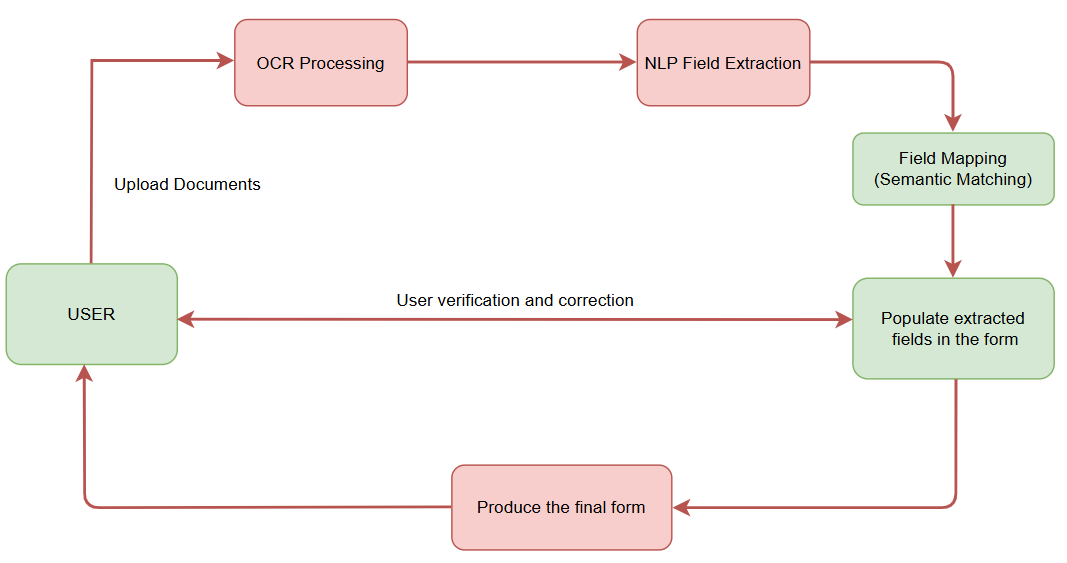
\includegraphics[width=\textwidth]{image/New/system.png}
    \caption{Architecture Diagram of the AI-Powered Code Documentation Generator.}
    \label{fig:architecture}
\end{figure}
\FloatBarrier



\section{Data Flow Diagram (DFD)}
\hspace{0.5cm}Figures 5.2 and 5.3 illustrate the data flow diagrams of the proposed system, showing the complete movement of data throughout the automated code documentation generation process.
\subsection{DFD Level 0}

\hspace{0.5cm}Figure 5.2 demonstrates the Level 0 Data Flow Diagram (DFD) of the AI-Powered Code Documentation Generator. The user provides source code to the system, which uses AST analysis to extract essential details such as functions, classes, imports and other relationships. Based on this extracted information, the AI generates structured documentation and delivers it to the user.
\hspace{0.3cm}
\FloatBarrier
\begin{figure}[h]
	\centering
	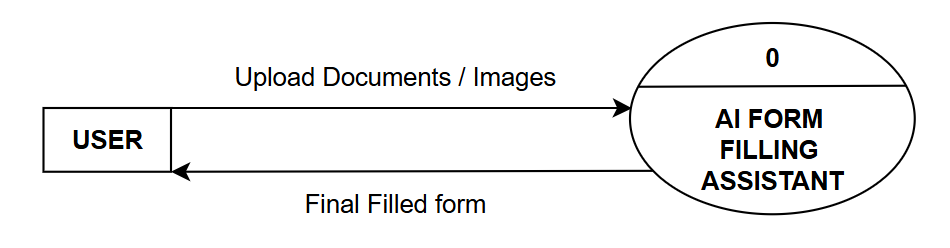
\includegraphics[scale=0.6]{image/New/dfd0.png}
	\caption{Data Flow Diagram Level 0.}
	\label{lvmh2}
\end{figure}
\subsection{DFD Level 1}


\hspace{0.5cm}Figure 5.3 presents the internal processing of the AI-Powered Code Document Generator as a Level 1 DFD. The process begins when the user uploads the source code and the Language Detection Module identifies the programming language based on the file extension. Once the language is detected, two parallel streams occur: the Text Feature Extraction Module extracts textual information and code metrics, generating text data, while the AST Extraction Module parses the code to create its abstract syntax tree, representing its structural organization. The AST is then passed to the Graph Feature Extraction Module to produce graph-based features capturing relationships among functions, classes and method calls. All features are merged in the Feature Fusion Module, which is subsequently processed by the LLM Engine (Ollama) to generate a natural language description of the source code. Finally, the Document Generation Module formats this output into structured documentation for the user.

\hspace{0.3cm}
\FloatBarrier
\begin{figure}[htbp]
    \centering
    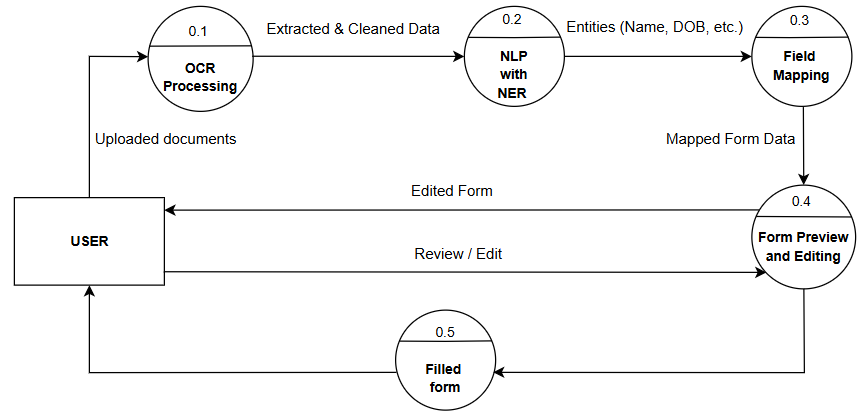
\includegraphics[width=\textwidth,keepaspectratio]{image/New/dfd1.png}
    \caption{Data Flow Diagram Level 1.}
    \label{fig:dfd1}
\end{figure}

\newpage


\section{List of Modules}
\hspace{0.5cm}
The AI-Powered Code Documentation Generator is composed of the following modules:
\begin{itemize}
    \item User Interface Module
    \item Language Detection Module
    \item Text Feature Extraction Module
    \item AST Analysis Module
    \item Graph Building Module
    \item Feature Fusion Module
  
    \item LLM Engine Module
    \item Documentation Output Module
\end{itemize}

\newpage
\subsection{User Interface Module}
\hspace{0.5cm}
This module serves as the main interface between the user and the system. It allows users to provide source code files, project directories or repository URLs and access both the generated documentation and the results of intermediate analysis. The interface ensures smooth navigation through each step of the process, making the analysis workflow seamless for the user.

\subsection{Language Detection Module}
\hspace{0.5cm}
The Language Detection Module identifies the programming language of the uploaded source code by analyzing file extensions and syntax. This detected language guides the system in selecting the appropriate parsing strategies and analysis methods. Accurate identification ensures correct AST generation and feature extraction, allowing the system to efficiently process multi-language projects and improving overall flexibility and adaptability.

\subsection{Text Feature Extraction Module}
\hspace{0.5cm}
This module extracts text-based features from the source code, calculating metrics such as the number of lines, tokens, comments, identifiers and keywords. It also identifies import statements, revealing external libraries and dependencies used in the project. These features are critical for generating project-level documentation, including README files and technology stack summaries, providing a comprehensive overview of the codebase. The module operates independently of language-specific syntax, making it fast and lightweight.

\subsection{AST Analysis Module}
\hspace{0.5cm}
This module analyzes the structure of the source code using an AST. It provides detailed insights into the internal structure of the code by extracting classes, functions, parameters, return types, variables, imports and function calls. As a core module, it ensures accurate and meaningful documentation based on the code itself rather than assumptions. It also supports language-aware analysis to enhance extraction accuracy and efficiency.

\subsection{Graph Building Module}
\hspace{0.5cm}
This module constructs a semantic graph from the AST. Nodes represent code elements such as files, classes and functions, while edges indicate relationships like function calls, imports and inheritance. The graph provides a clear visualization of interactions among code components, illustrating data flow and module dependencies. It also supports deeper analysis, including the identification of recursion, unused functions and critical components.

\subsection{Feature Fusion Module}
\hspace{0.5cm}
This module integrates textual features, AST-based structural features and graph-based relational features. Textual features provide specific information, AST features detail the functionality of each component and graph features illustrate the relationships between components. By combining all these features, the system can generate more accurate and comprehensive documentation, ensuring that no information is lost during processing.

\subsection{LLM Engine Module}
\hspace{0.5cm}
This module uses a LLM to create human-readable documentation. The input to the module consists of feature summaries created from the AST, text and graph analysis. The model uses the structural and contextual information to create accurate documentation about the functionality of the code and the architecture of the system. This ensures the readability, accuracy and appropriateness of the created documentation. The level of detail in the documentation depends on the complexity of the input code.

\subsection{Documentation Output Module}
\hspace{0.5cm}
This module handles structuring the generated documentation in an organized layout, covering areas such as project overview, architecture, API documentation and module-level details. It ensures consistency in presentation, enhancing readability and usability. The documentation can be exported to formats like Markdown, making integration with existing development workflows easier and supporting efficient sharing and management.
\newline
\par In this chapter, the overall system design of the AI-Powered Code Documentation Generator is discussed, including the system architecture, the functionality of its various modules and the complete data flow. This design enables each module to process the source code independently while ensuring that the analysis and documentation generation proceed systematically and cohesively. With the system’s design and architecture established, the next chapter will cover the implementation aspects, detailing the development of each module and how they integrate to achieve the intended functionality.

\chapter{SYSTEM IMPLEMENTATION}
\hspace{0.5cm}
The system implementation phase is aimed at realizing the AI-Powered Code Documentation Generator design. At this stage, full development occurs, including the implementation of all system modules, such as the code parser, structural feature extraction algorithm, semantic understanding algorithm and automatic documentation generator. Each module is developed and implemented independently, allowing developers to make changes or enhancements without affecting other modules. This approach ensures high scalability, as modifications and additions can be implemented easily while maintaining the integrity and efficiency of the system.
\section{Setup Development environment}
\hspace{0.5cm}The importance of having an efficient development environment cannot be ignored when implementing and executing the system. In the context of the current system, the VS Code editor is chosen as the development environment for its lightweight structure and easy integration with different tools. The backend is designed with the Python 3.8 language because of the numerous benefits that come with the use of this language when processing data and implementing machine learning algorithms. The HTML (HyperText Markup Language), CSS (Cascading Style Sheets) and JavaScript languages are used to implement the frontend of the system to make the interaction experience of the user more engaging. The backend server has been implemented using the Flask web framework, which helps in creating RESTful APIs for the smooth communication between the frontend and backend modules.
To support the implementation of various functionalities, the following Python libraries are installed and configured:\begin{itemize}
\item \textbf{Flask} -- This tool is used in constructing the backend server as well as the REST (Representational State Transfer) API endpoints. It manages all requests made by users, like uploading files. This too starts the code analysis and sends back the documentation that is created.

\item \textbf{Tree-sitter} -- This tool is used for parsing source code and converting it into ASTs, enabling accurate syntactic analysis for multiple programming languages. It divides the source code into structural elements such as functions, classes and other components.

\item \textbf{Tree-sitter-languages} -- This library provides built-in language support that extends Tree-sitter’s capabilities, allowing the system to support multiple programming languages such as Python, Java, JavaScript, C, C++, Go, Rust and Kotlin without the need for separate parser configurations for each language.

\item \textbf{Markdown} -- A Markdown library provides tools to parse, render and manipulate Markdown content programmatically.  
Such libraries support creating dynamic documentation, reports or web content from plain text. 
They simplify integrating Markdown-based documentation into automated systems and applications.

\item \textbf{Networkx} -- This tool is used to construct and analyze graph structures derived from the parsed code helping to achieve a deeper contextual understanding of the code.
\end{itemize}
\section{User Interface}
\hspace{0.5cm} The User Interface is built as a single-page application with HTML, CSS and JavaScript, enabling users to upload source code files, folders or even input a public Git repository URL. The User Interface supports three modes: Single File, Folder and Mixed.

\par The frontend sends a request to the \textit{/analyze} endpoint to communicate with the Flask-based backend. Once the request is received, the backend will process the input by calling the core function \textit{analyze\_path()}. This function will determine whether the input is a file, folder or Git URL and then route it to the appropriate analysis pipeline. If it is a Git URL, the repository will be cloned to a temporary directory and then cleaned up. If it is a local input, the function will directly call either the single-file analysis pipeline or the project-level analysis pipeline based on whether the path is pointing to a file or a directory.

\par The generated documentation will be displayed in the browser as formatted HTML using the marked.js library. Users will also be able to download the complete generated Markdown files as a ZIP package using the JSZip library.

\section{Language Detection}
\hspace{0.5cm}
The next step is to recognize the programming language of each uploaded source file based on its file extension. This is done by utilizing an extension-to-language mapping defined in \textit{language\_config.py}, which allows the system to support twelve programming languages including Python, Java, JavaScript, TypeScript, C, C++, Go, Rust, PHP, Ruby, Kotlin and C\#.

\par During processing, the file extension is extracted from the file path, which is converted to lowercase for standardization purposes, as different operating systems have different capitalization standards. After that, the programming language is detected based on the predefined file extension mapping.

\par In order to ensure robustness, the unsupported file types will be skipped during the traversal of the folders. Also, empty files will be removed prior to the start of the analysis process. Moreover, the Git metadata directories such as \textit{.git} will be skipped during the traversal of the folders using the normalized paths where backslashes will be replaced with forward slashes in order to support both the Windows and Linux platforms, thus preventing the Git source code from being treated as source code.

\section{Text Feature Extraction}
\hspace{0.5cm}
In this stage, lightweight textual features are obtained from individual source files without reference to the AST, aiming to identify basic structural properties of the code. The features are calculated through text-based analysis in \textit{text\_features.py} without any reference to language parsing or grammar.

\par The function reads the source file in a safe manner with UTF (Unicode Transformation Format)-8 encoding and ignores decoding errors for robustness across different file types and legacy codebases. In case the file is invalid or cannot be read, an empty dictionary is returned.

\par The features that are extracted are the raw counts, which include the total number of lines, the total number of characters, the number of import statements, the number of class definitions and the number of function definitions. These features offer an overview of the source file.

\par These metrics are attached to every function record as a \textit{metrics} field. They help in the formation of the unified fused representation in the downstream modules.

\section{AST Analysis}
\hspace{0.5cm}
In this stage, structural information is obtained through structural feature extraction, where each source file is parsed to an AST with the help of the tree-sitter framework, facilitating precise analysis for all fourteen programming languages.

\par The entry point is \textit{tree\_sitter\_adapter.py} where the programming language is resolved based on the file extension, the source file is read in a safe manner with UTF-8 encoding and the parse tree is generated along with a source representation at the byte level to accurately extract the text within nodes. Node type names such as function definitions, class declarations and call expressions for different languages are read from \textit{language\_config.py} to ensure that the logic itself doesn’t have any explicit language checks.

\par The AST is processed in \textit{ast\_graph.py} with a two-pass strategy. The first pass traverses the entire AST tree structure to collect all the function names, class names and import symbols in the \texttt{known\_names} set. The \textit{known\_names} set will be used in the second pass of the AST traversal process to differentiate calls to functions defined within the project codebase from calls to external library code. The \textit{known\_names} set is supplemented with symbols obtained from all the files in the codebase in the global pre-pass in \textit{analyzer.py}.

\par The second pass carries out full per-function extraction. For a function, the system extracts the function's name, class membership, parameters, return type, internal function calls, external function calls, local variables and string literals. For function names, a four-strategy cascade is used to accommodate the different structural characteristics of programming languages. Most languages rely on a direct field lookup for function names, while the languages C and C++ rely on a declarator chain walk and a shallow identifier scan and a deep recursive scan serve as a fallback.

\par Although function calls are identified during this process, the caller-callee relation is not stored as a string. Rather, every identified internal call is directly added to the NetworkX graph by invoking \textit{graph.add\_edge()}. This graph is the sole source of all call relation data. The extracted function-level metadata is stored in the \textit{metadata} dictionary and passed to the next stage, Graph Analysis.


\section{Graph Analysis}
\hspace{0.5cm}
Within this stage, the semantic graph created during the AST traversal process is examined to determine higher-level structural information about the codebase. The graph is built using the NetworkX library, in which the nodes of the graph represent the functions and the edges represent the caller-callee relations. The graph is the single source of truth for all call relationship data, which means the data about the relations of the functions is not obtained from intermediate lists of strings or the AST.

\par The call relationships in the graph are obtained by using successor queries on the graph, where the outgoing edges on a function node directly provide the list of functions it calls. This method ensures consistency throughout the system and avoids the need for string parsing and redundant storage.

\par In addition to storing the relationships between the entities, the graph is used to find four different structural characteristics in the code. The entry points in the code are the set of functions that have no incoming edges but have outgoing edges; in other words, these are the functions that are never called by any other function in the code but start the calls themselves. The dead functions in the code are the set of functions that have neither incoming nor outgoing edges; in other words, these are the functions that are never called in the code and never start any calls either. A cross-file check is done before determining the dead or entry point functions in the code.

\par Direct recursion is identified through self-loop edges in the graph, where a function has an edge pointing back to itself. Mutual and chain recursion are detected using cycle detection algorithms, which identify groups of functions forming circular call chains of length greater than one. Critical functions are determined by ranking nodes based on their in-degree, where functions with a higher number of incoming edges are considered the most depended-upon in the codebase.
\par These features of the derived graphs are included in each function’s record and passed on to the Feature Fusion and Documentation Generation stages, which enrich the LLM prompt with architectural information that cannot be automatically inferred from the AST features.

\section{Feature Fusion}
\hspace{0.5cm}
At this stage, features extracted by the Text Feature Extraction, AST Analysis and Graph Analysis modules are integrated into a single structure for each function. This integration encompasses the structural, relational and contextual aspects of the code in a single structure, which is used by all the modules.

\par The fusion is achieved in \textit{analyzer.py} through the \textit{\_build\_record()} function, which constructs one record per function by combining three different sources of information. The information from the AST is used for the structural facts about each function, including its name, its membership in a class, parameters, return type, external calls, local variables, string literals and imports. The information from the graph is used for the relational facts, including the list of internal calls and the formatted caller-callee relationship strings, both of which are obtained directly from graph successor queries. The text features include the contextual metrics, including the raw counts used by the LLM..

% \par The graph acts as the single source of truth for all call relationship data throughout the fusion process. Rather than storing call relationships as strings during the AST walk, they are derived at record construction time by querying the graph, which eliminates redundancy and ensures that the relationships stored in the record always reflect the actual graph structure.

% \par The complete graph analysis result from \texttt{analyze\_graph()} is also embedded in each function record. This includes entry points, dead functions, direct recursion, mutual cycles, most critical functions, and the longest execution path — all of which are used in the documentation generation stage to provide architectural context to the LLM.

\par The resulting fused records are serialized into \textit{semantic\_records.json}, which is used as the persistent interface between the analysis pipeline and the module for generating the documentation.


\section{Documentation Generation}
\hspace{0.5cm}
The Documentation Generation Module uses the open-source LLM DeepSeek, which is hosted locally via Ollama, to create structured Markdown documentation from the integrated code records. The model is accessed via the Ollama HTTP API with a low temperature of 0.1 to ensure consistent and factually reliable outputs. The \textit{stream: false} parameter ensures that the complete response is returned as a single JSON (JavaScript Object Notation) payload, simplifying downstream processing.

\par For each function, a structured fact block is created from the fused record and passed into the LLM as a prompt. This fact block combines all three sources of features into one line of context.


\par All documents are generated in parallel by a \textit{ThreadPoolExecutor} with up to six concurrent workers, greatly improving the total generation time for large projects. If a document does not generate correctly, it will have a stub so that the pipeline always produces a complete output even in the presence of individual failures


\par The module produces four types of Markdown documentation artifacts per run of the analysis:
\begin{itemize}
\item \textbf{README.md} for project overview, description, tech stack, project structure, etc.
\item \textbf{architecture\_overview.md} for component responsibilities, data flow between files, module dependencies, etc.
\item \textbf{File-wise .md files} for file-wise information like import information, member variables, function intents, parameters, return types, function call relationships, entry points, dead code, recursion and cycles.
\item \textbf{recent\_changes.md} for displaying Git commit history with author information and message for every commit, if input is provided as a Git repository URL.
\end{itemize}

\par The implementation phase has been successfully completed to transform the proposed design into a fully functional form of the AI-Powered Code Document Generator. All the modules, ranging from language detection and AST parsing to graph analysis, feature fusion and LLM-based generation, have been implemented and integrated to function cohesively in a complete system. Since the system has been fully operational for a range of programming languages and input types, the discussion will move on to the evaluation stage. The next chapter will cover the results achieved by running the system on a range of projects and a discussion on the quality, accuracy, and completeness of the generated documentation.

% \begin{lstlisting}[language=python]
% from sentence_transformers import SentenceTransformer, util

% model = SentenceTransformer('all-MiniLM-L6-v2')

% def map_profile_to_form(profile, form_fields):
%     mapped = {}
%     for field, value in profile.items():
%         best_match = None
%         best_score = -1
%         for form_field in form_fields:
%             score = util.cos_sim(
%                 model.encode(field, convert_to_tensor=True),
%                 model.encode(form_field, convert_to_tensor=True)
%             )
%             if score > best_score:
%                 best_score = score
%                 best_match = form_field
%         mapped[best_match] = value
%     return mapped
% \end{lstlisting}

% \section{Form Auto-Filling}
% \hspace{0.3cm}
% The final mapped data is converted to JSON and sent to the frontend. 
% A JavaScript script runs on page load to automatically fill the form fields 
% with the extracted details.

% \begin{lstlisting}[language=javascript]
% <script>
%   const filledData = {{ final_form_data | tojson }};
%   window.onload = () => {
%     for (let key in filledData) {
%       const el = document.querySelector(`[name="${key}"]`);
%       if (el) el.value = filledData[key];
%     }
%   };
% </script>
% \end{lstlisting}


% \hspace{0.3cm} This module-based implementation ensures flexibility to add more document types in the future while keeping extraction accurate and rule-based.

% Thus, the system completes the pipeline: document upload $\rightarrow$ 
% text extraction (PDF-first, OCR for images if required)$\rightarrow$ field extraction $\rightarrow$ consolidation $\rightarrow$ 
% form field mapping $\rightarrow$ auto-filling.
\chapter {RESULTS AND DISCUSSION}
\hspace{0.5cm}
This chapter presents and analyzes the results obtained from the proposed system, the AI-Powered Code Documentation Generator. The system was evaluated using source code files provided through two input methods: direct file uploads via the web interface and repository-based inputs through public Git URLs. This dual-mode testing ensured that the system was assessed under both isolated and real-world development scenarios.

The results demonstrate that the system is capable of effectively processing multi-language codebases and generating well-structured, coherent and contextually relevant documentation. By integrating techniques such as syntactic analysis, structural feature extraction and language model-based generation, the system successfully transforms raw source code into meaningful documentation. Overall, the observed outputs highlight the system’s reliability, scalability and practical applicability in automating documentation tasks across diverse programming environments..

\section{Results}
\hspace{0.5cm}The system was tested in different input modes to evaluate its functionality and output quality. The following figures illustrate the working of the system and the documentation generated at various stages.
\par The screenshot in Figure 7.1 displays the homepage of the AI-Powered Code Documentation Generator when in file upload mode. There are two modes in which a user can input the source code. These modes are Upload Files and Repository URL.
\vspace{1cm}
\FloatBarrier
\begin{figure}[h]
	\centering
	\fbox{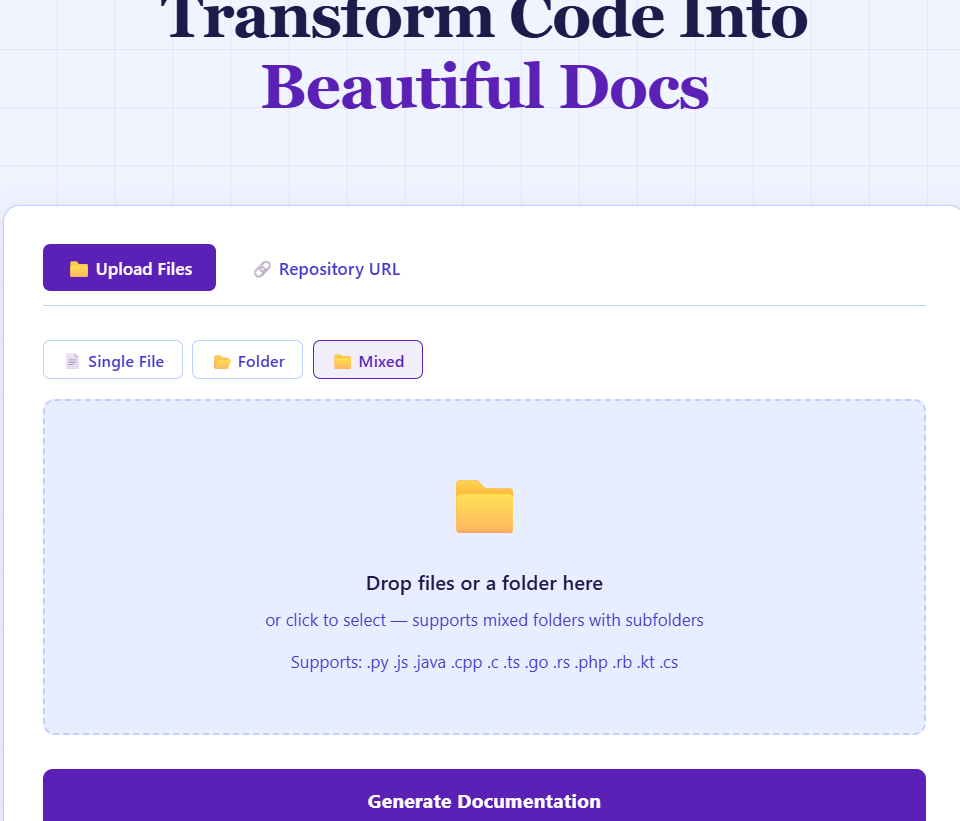
\includegraphics[width=0.6\textwidth]{tex/Screenshot 2026-04-14 215024.png}}
	\caption{Complete User Interface of the System.}
	\label{lvmh2}
\end{figure}
\FloatBarrier

\vspace{1cm}
\begin{figure}[h]
	\centering
	\fbox{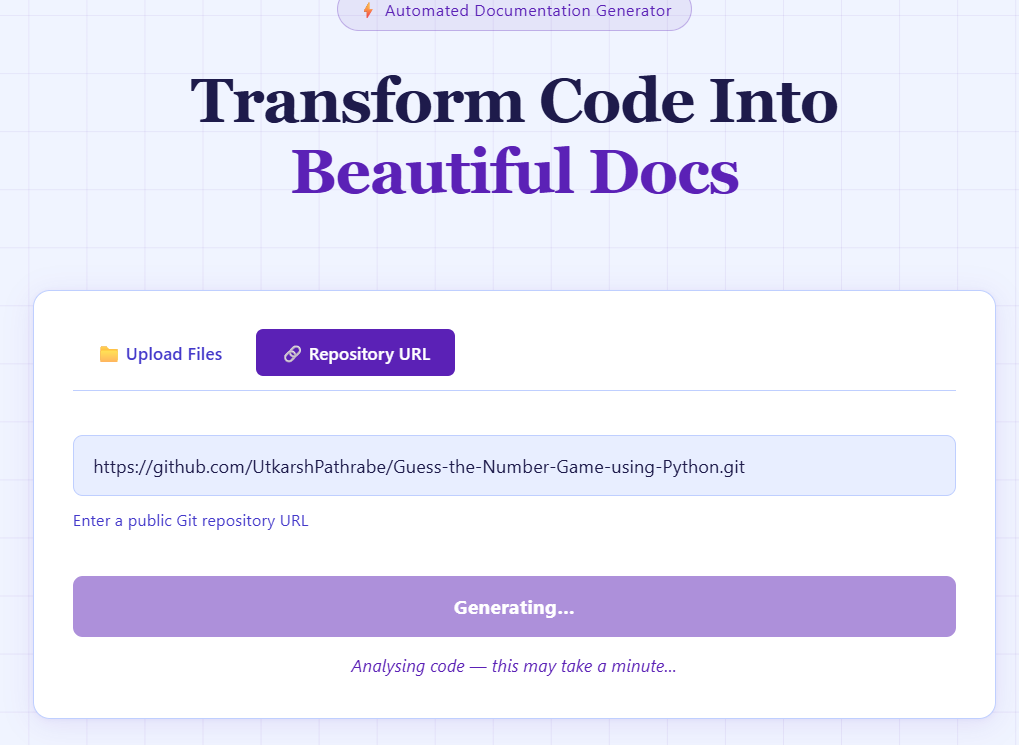
\includegraphics[width=0.6\textwidth]{tex/Screenshot 2026-04-16 072516.png}}
	\caption{Home Page – Repository URL Input Mode.}
	\label{lvmh2}
\end{figure}
\FloatBarrier

\par Figure 7.2 shows the User Interface (UI) for the homepage with the Repository URL mode selected. The user can provide the public git repository URL in the text box. The system then downloads the repository in a temporary directory and processes all the source files from the repository without the need to upload the files.

\vspace{1cm}
\FloatBarrier
\begin{figure}[h]
	\centering
	\fbox{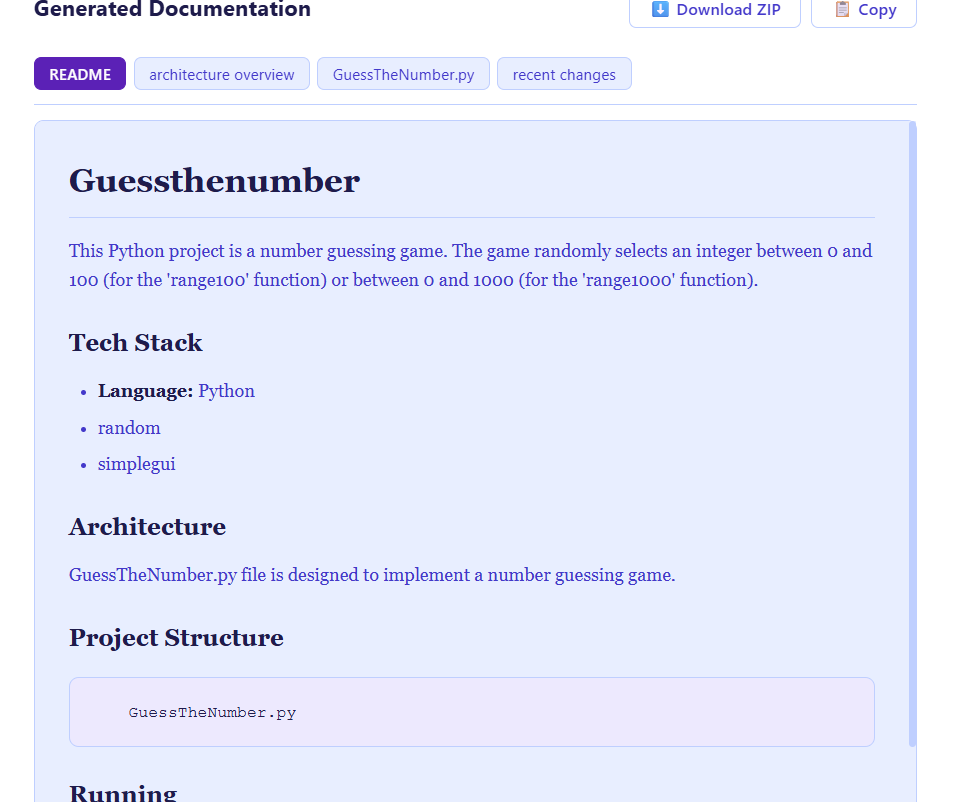
\includegraphics[width=0.6\textwidth]{tex/Screenshot 2026-04-16 073000.png}}
	\caption{README.md – Project Overview Output.}
	\label{lvmh2}
\end{figure}
\FloatBarrier

\par The system shows the README tab of the generated documentation output in Figure 7.3. It analyzes the repository and provides a project-level summary, including project description, technology stack, architecture summary, run instructions, and project structure.

\vspace{1cm}
\FloatBarrier
\begin{figure}[h]
	\centering
	\fbox{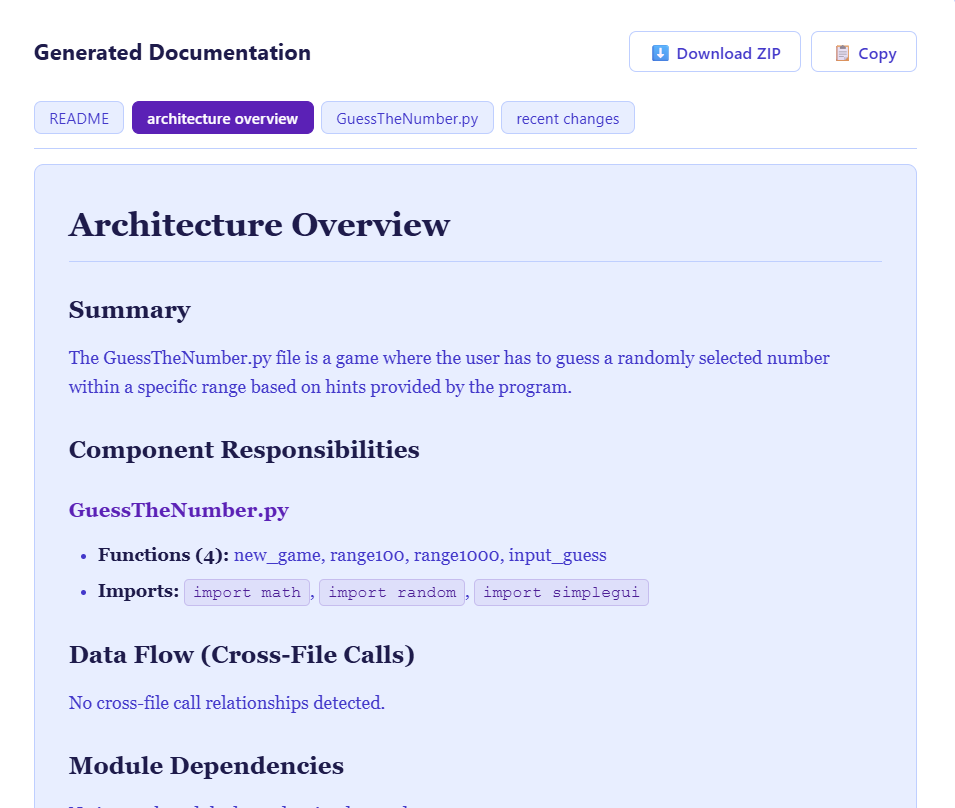
\includegraphics[width=0.6\textwidth]{tex/Screenshot 2026-04-16 073016.png}}
	\caption{architecture\_overview.md – Architectural Description Output.}
	\label{lvmh2}
\end{figure}
\FloatBarrier

\par Figure 7.4 shows the system displaying the Architecture Overview tab of the automatically generated documentation. The system generates a structured architectural description consisting of file-wise summary information, component responsibilities such as classes, functions, imports and fields, call relationships between files representing data flow and module dependencies from both import statements and function interactions.

\par Figure 7.5 shows the file-wise documentation generated for the application in Markdown format. Each file has its documentation with information like function intent, parameters, return values, function calls, local variables and internal call relationships, along with graph-based information like entry points, unused functions, dependencies and recursion information.

\vspace{1cm}
\FloatBarrier
\begin{figure}[h]
	\centering
	\fbox{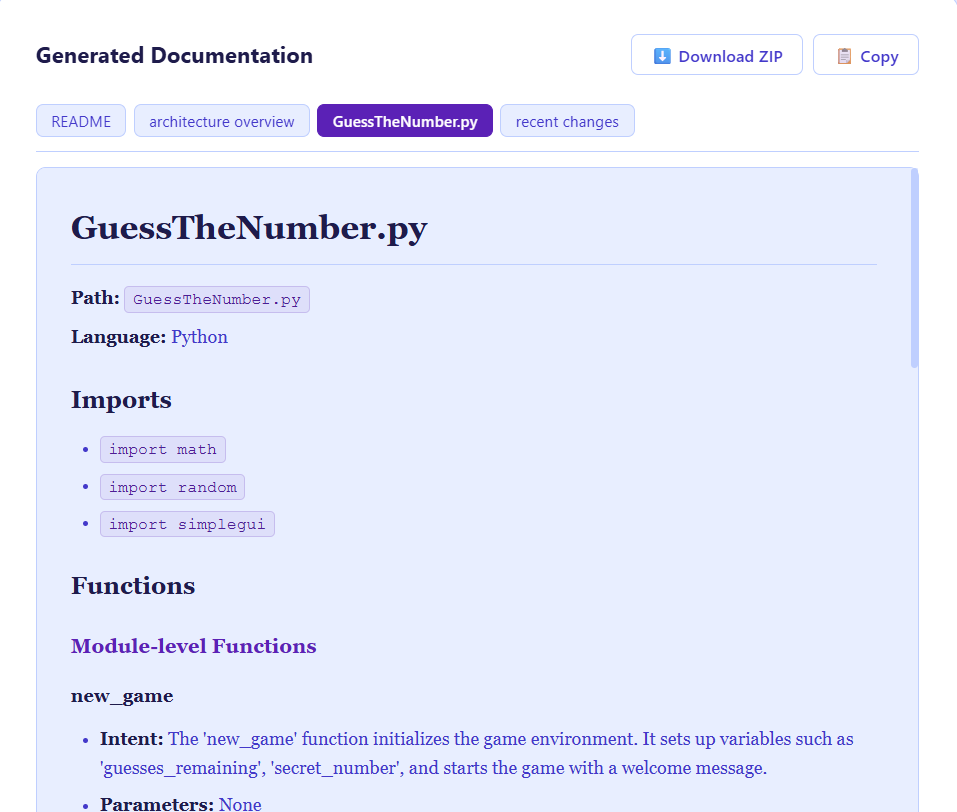
\includegraphics[width=0.6\textwidth]{tex/Screenshot 2026-04-16 073038.png}}
	\caption{File-wise .md Output.}
	\label{lvmh2}
\end{figure}
\FloatBarrier

\par Figure 7.6 shows the Recent Changes tab of the automatically generated documentation. The system has automatically collected the commit history from the Git repository and created a structured document named recent\_changes.md. This feature helps users easily track project updates and understand the evolution of the codebase over time.

\vspace{1cm}
\FloatBarrier
\begin{figure}[h]
	\centering
	\fbox{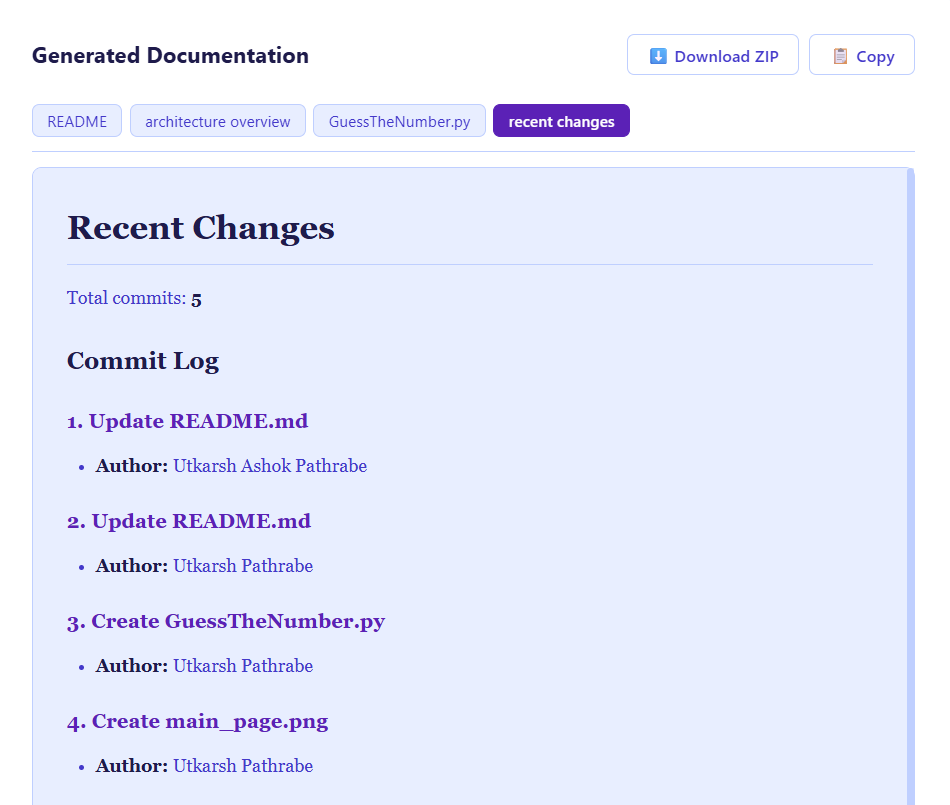
\includegraphics[width=0.6\textwidth]{tex/Screenshot 2026-04-16 073053.png}}
	\caption {recent\_changes.md – Git Commit History Output.}
	\label{lvmh2}
\end{figure}
\FloatBarrier

\section{Discussion}
\hspace{0.5cm}
The results show that the proposed system can efficiently produce overall documentation on different levels, including projects, architecture and functions. The accuracy in the extraction of structural information is guaranteed by AST-based analysis, while graph-based analysis allows for precise identification of relationships between functions. The inclusion of text-based metrics improves the results produced by the system, enhancing their overall relevance and readability.

\par The system works effectively with different programming languages, thus demonstrating the flexibility of the tool. This is further evidenced by the repository URL mode, which is beneficial since the entire projects can be analyzed without the need for file handling. Furthermore, the inclusion of the history of commits is advantageous since it provides additional information compared to other documentation tools.

\par However, the system is not without certain limitations. The quality of the code fed into the system will affect the quality of the documentation that is created. Also, the dynamic behavior of the code is not fully taken into consideration in the system. Nevertheless, the system is useful in reducing the effort required in understanding the code.

% The following figure shows the evaluation of reference audio and test audio by aligning note sequences of both. The green-colored notes represent correct notes. The blue-colored notes are the notes in reference audio missed by test audio. The red-colored notes represent the wrong notes in the test audio. 
% \vspace{1cm}
% \FloatBarrier
% \begin{figure}[h]
% 	\centering
% 	\fbox{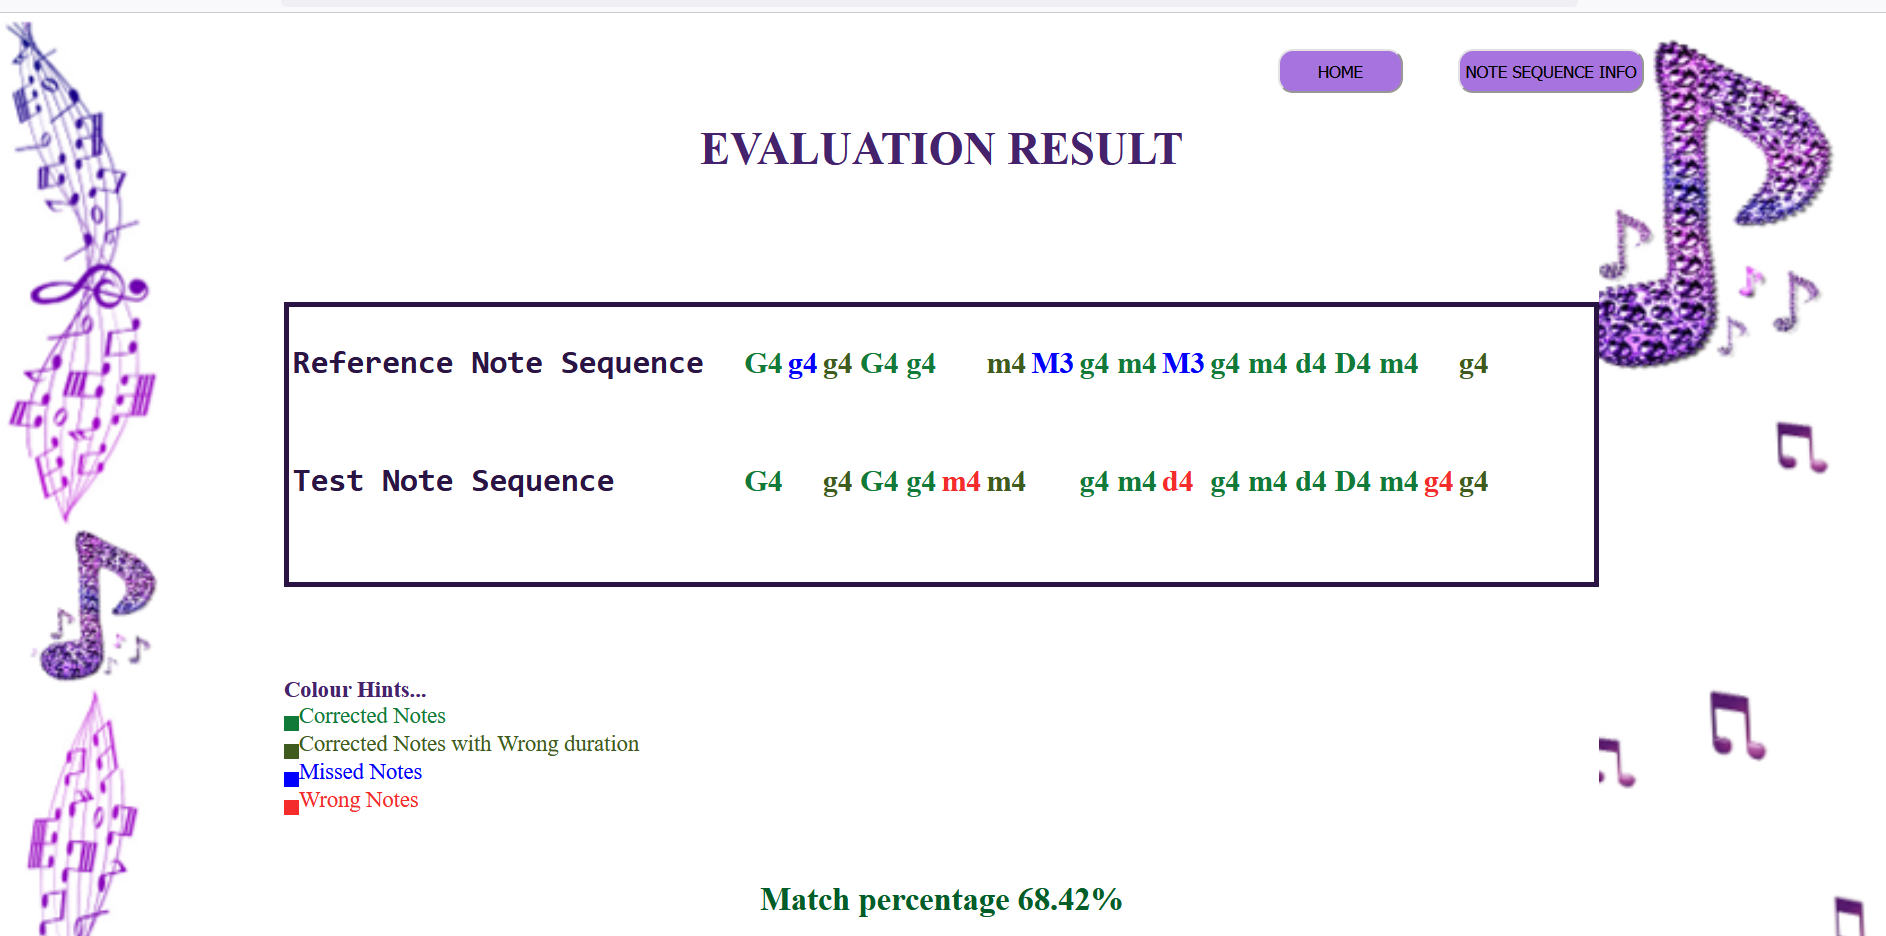
\includegraphics[scale=.27]{image/r6.png}}
% 	\caption{Evaluated Notes sequences}
% 	\label{lvmh2}
% \end{figure}
% \FloatBarrier
% % In the following figure show the play back of audio piece correspond to the selected note sequence part. the yellow colored notes are selected by user  for playback. when click  on it a play button is displayed. by click play button the play back can be done.
% %  \vspace{1cm}
% % \FloatBarrier
% % \begin{figure}[h]
% % 	\centering
% % 	\fbox{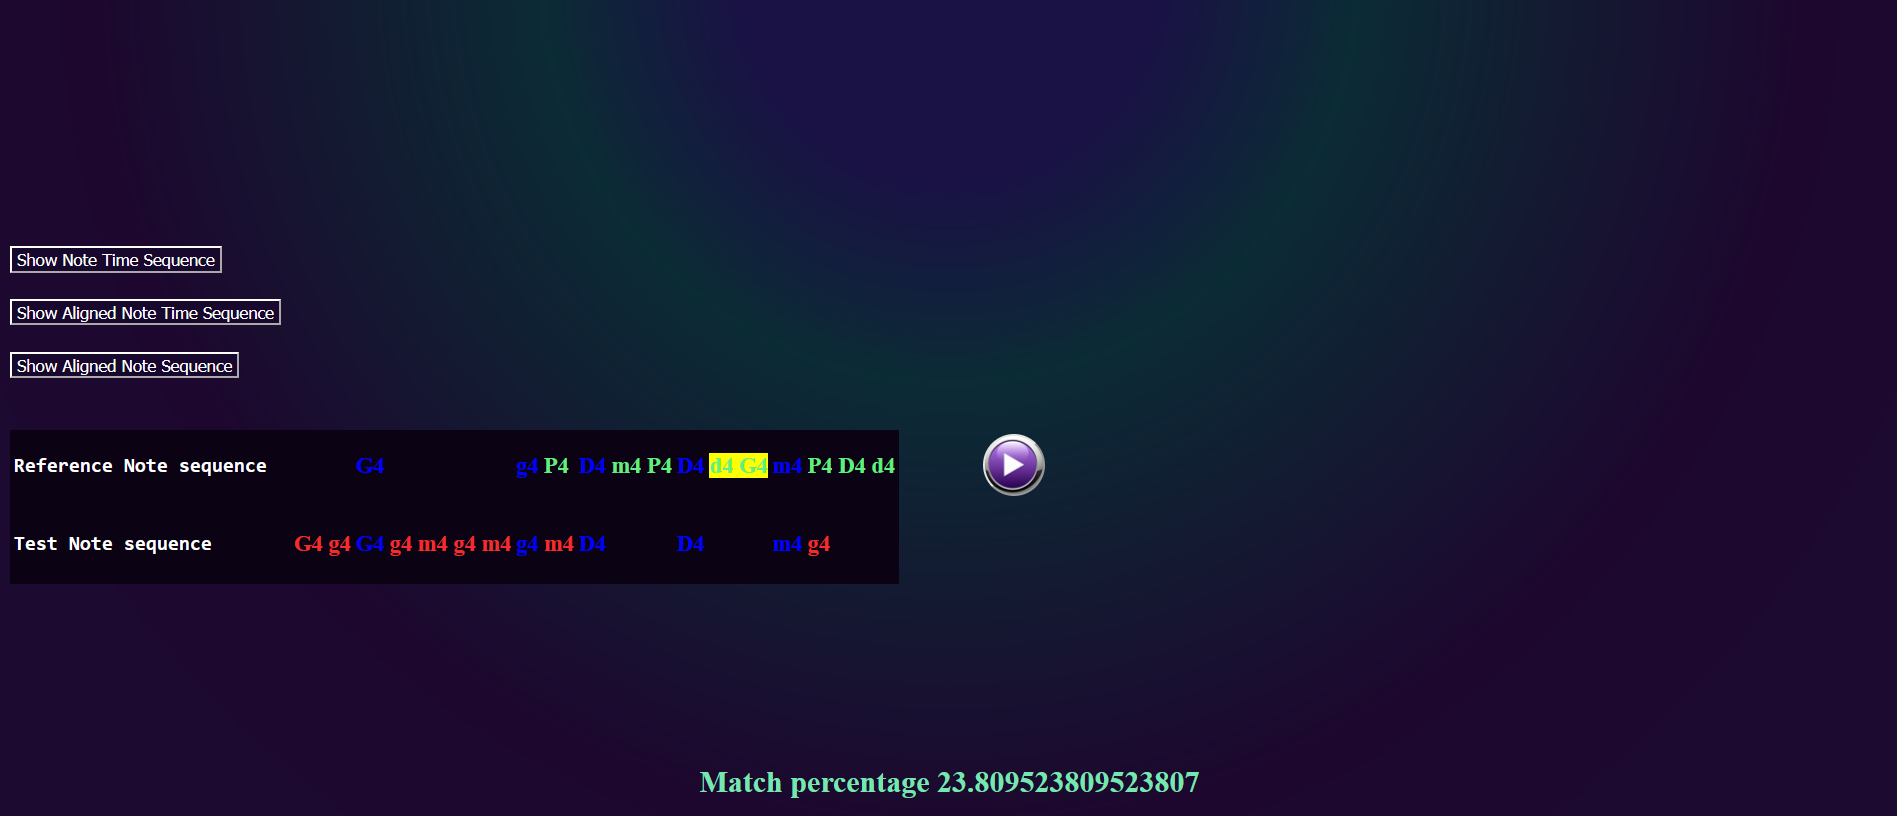
\includegraphics[scale=.27]{image/result7.png}}
% % 	\caption{Result 7}
% % 	\label{lvmh2}
% % \end{figure}
% % \FloatBarrier
% In the following figure, two play buttons are displayed to playback audio of selected note sequence pieces.
% \vspace{1cm}
% \FloatBarrier
% \begin{figure}[h]
% 	\centering
% 	\fbox{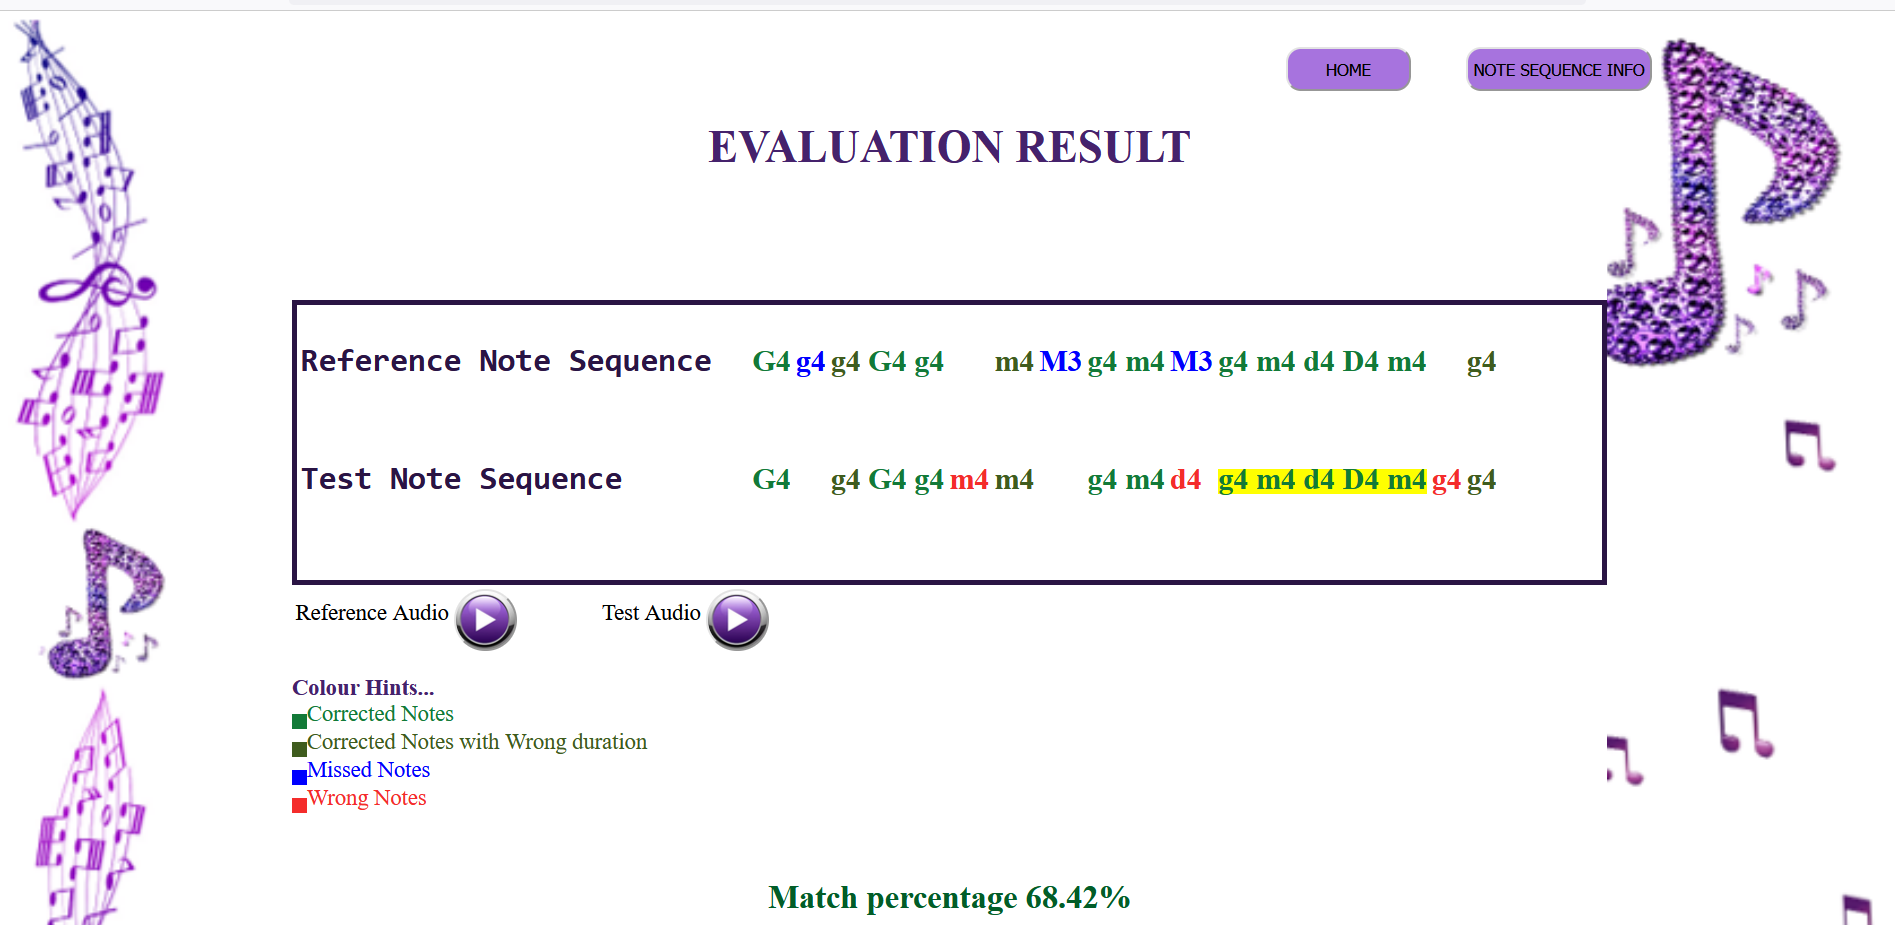
\includegraphics[scale=.27]{image/r7.png}}
% 	\caption{display play buttons on select note sequence peice}
% 	\label{lvmh2}
% \end{figure}
% \FloatBarrier

% % \vspace{1cm}
% % \FloatBarrier
% % \begin{figure}[h]
% % 	\centering
% % 	\fbox{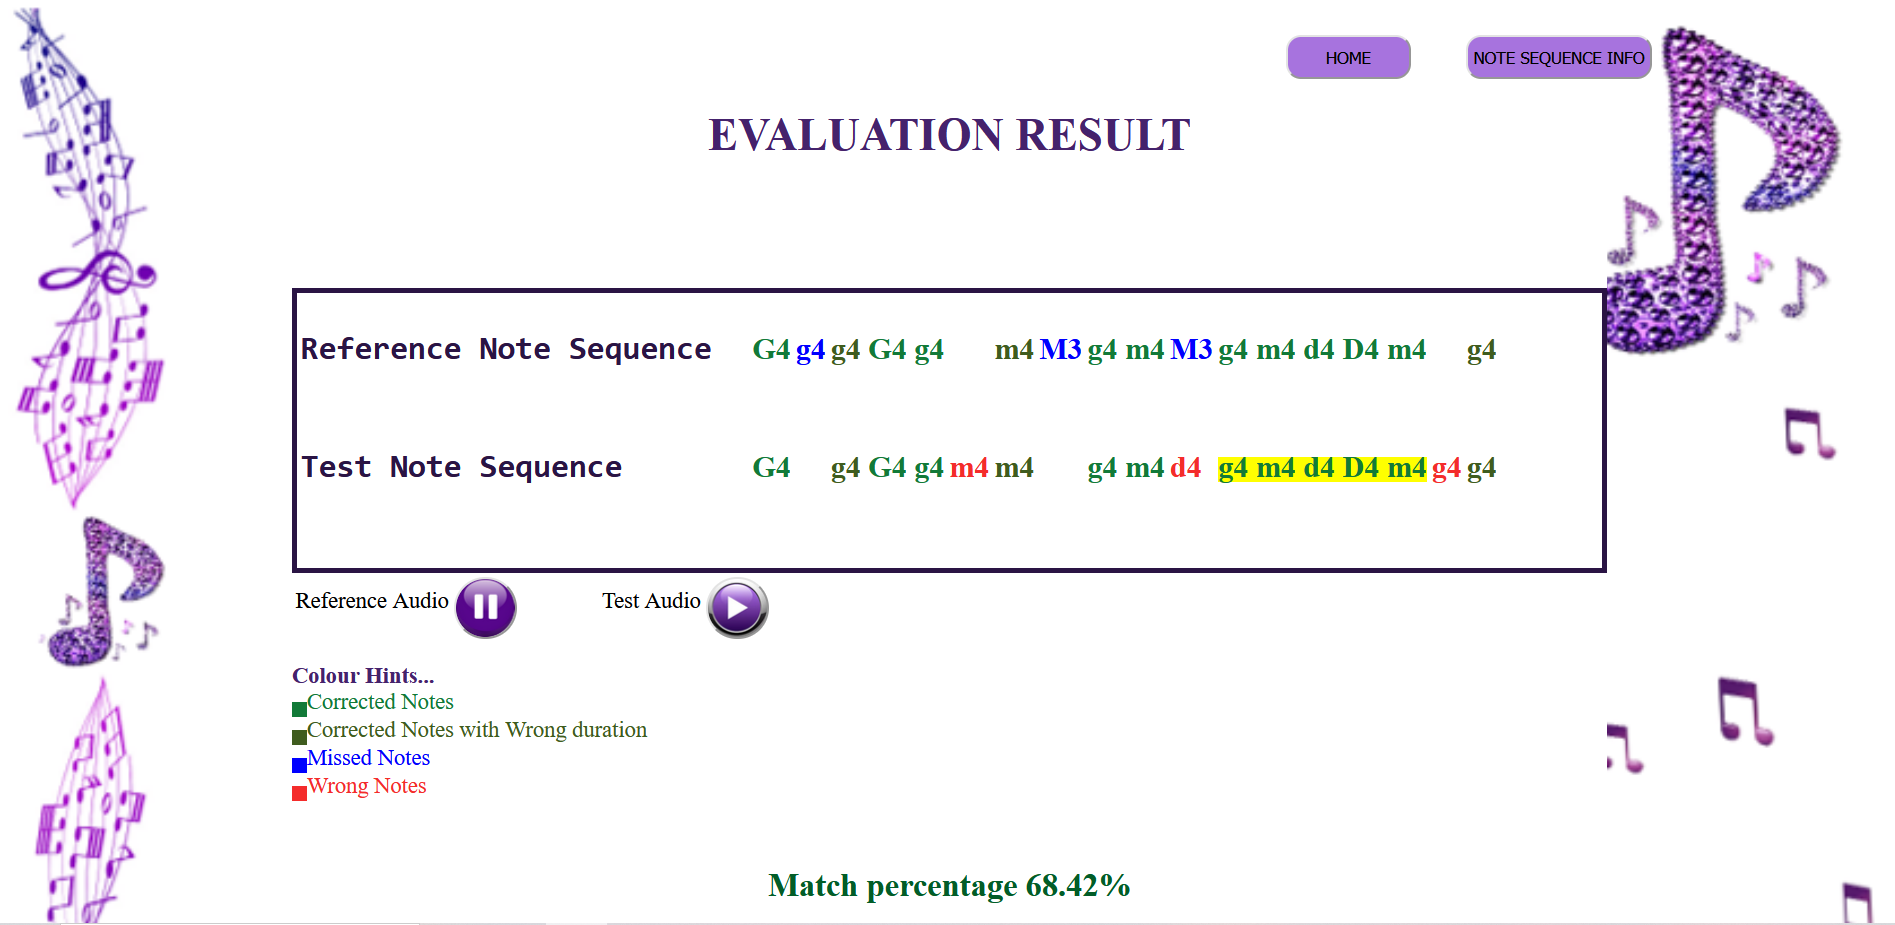
\includegraphics[scale=.27]{image/r8.png}}
% % 	\caption{play back of reference audio}
% % 	\label{lvmh2}
% % \end{figure}
% \FloatBarrier
% The following figure demonstrates inputting reference audio by recording audio using the record button displayed on the interface. Similarly, the test audio can also be recorded in the same manner.
% \vspace{1cm}
% \FloatBarrier
% \begin{figure}[h]
% 	\centering
% 	\fbox{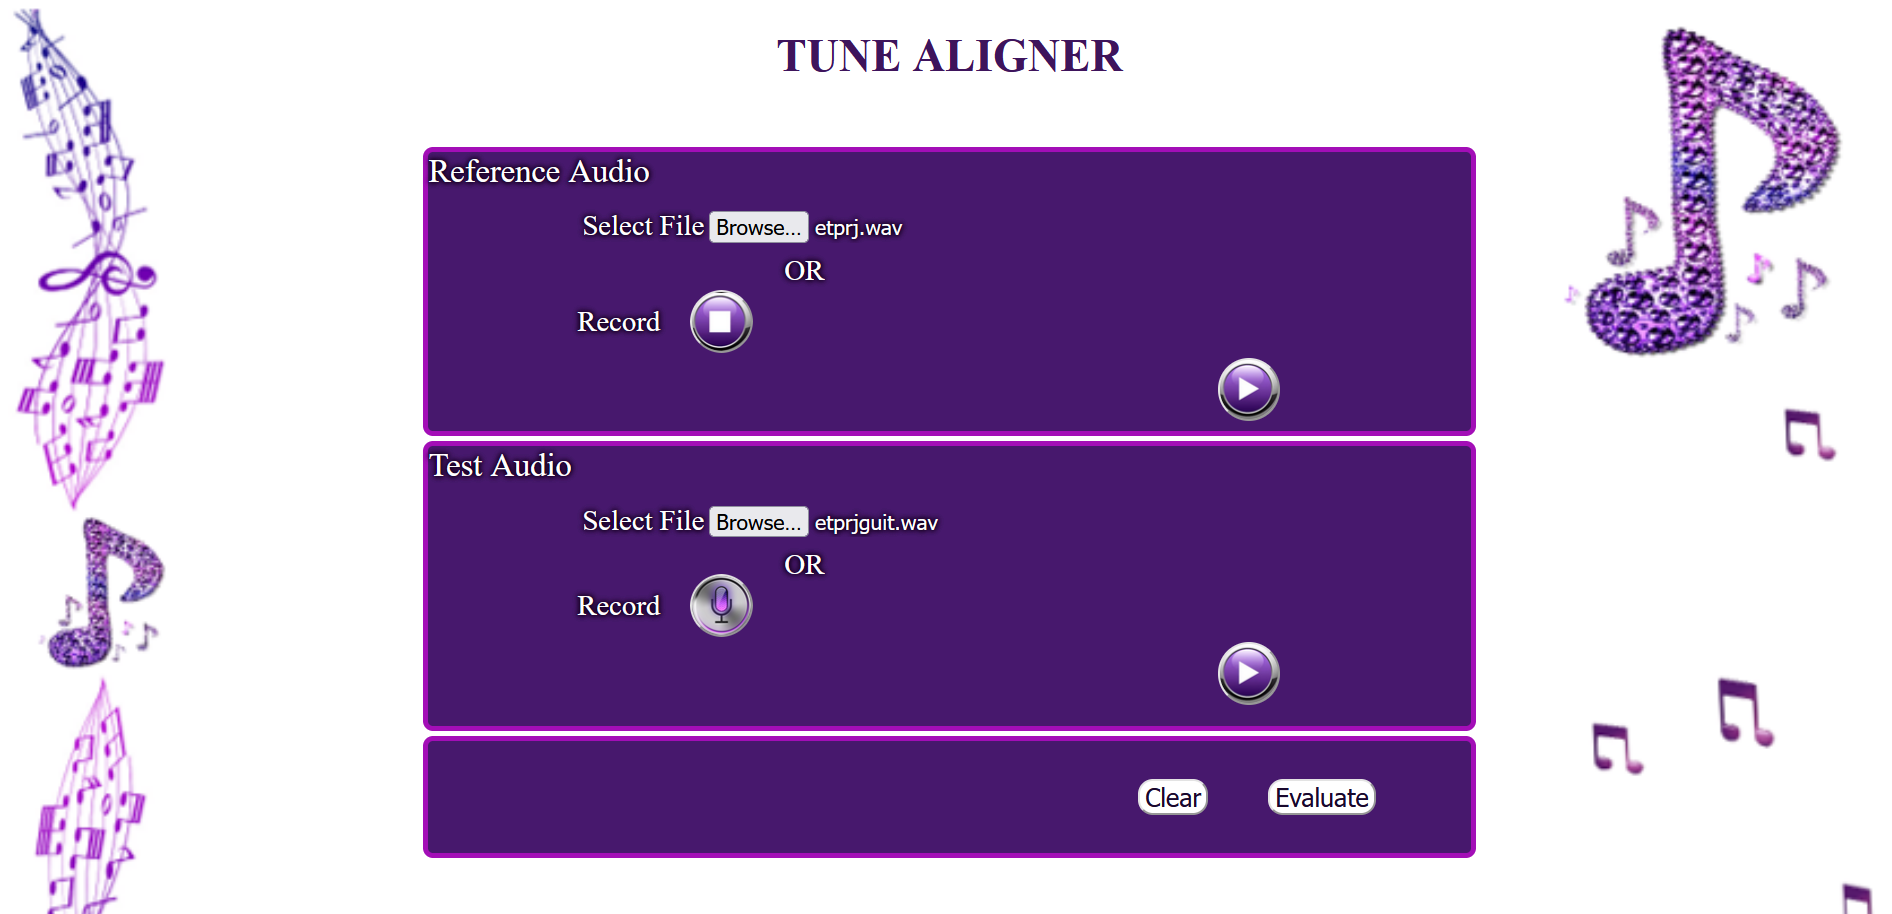
\includegraphics[scale=.27]{image/r9.png}}
% 	\caption{Record reference audio}
% 	\label{lvmh2}
% \end{figure}
% \FloatBarrier

% %  \vspace{1cm}
% % \FloatBarrier
% % \begin{figure}[h]
% % 	\centering
% % 	\fbox{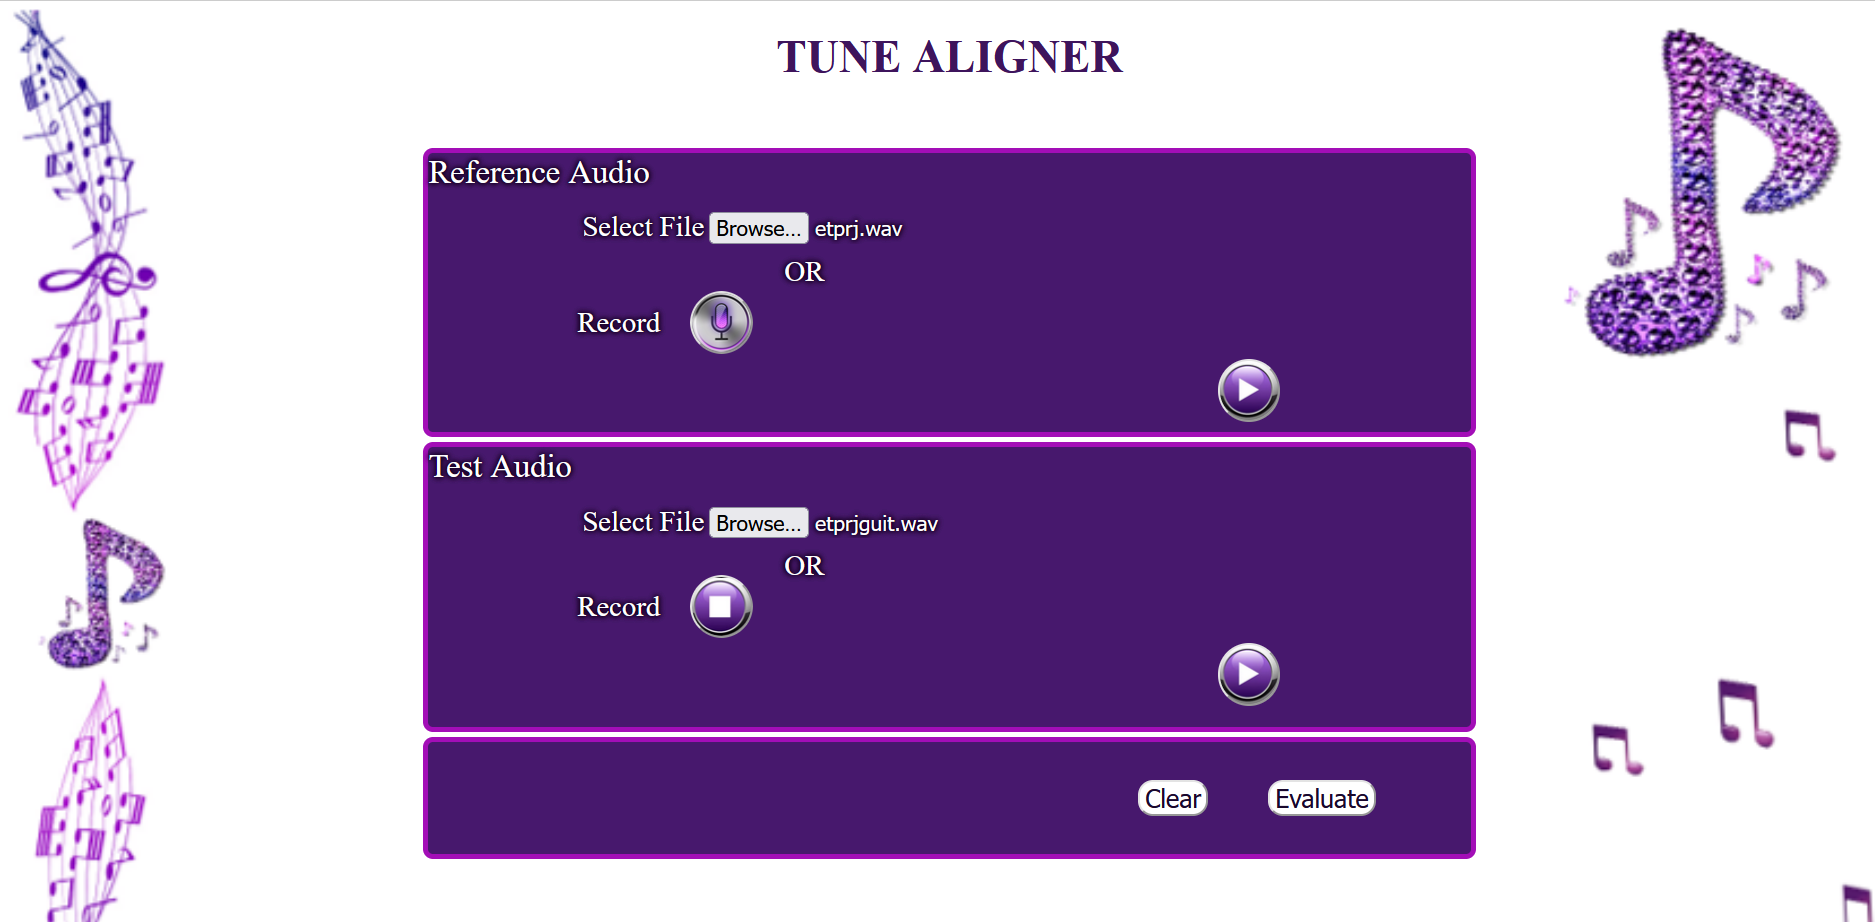
\includegraphics[scale=.27]{image/r10.png}}
% % 	\caption{Record Test audio}
% % 	\label{lvmh2}
% % \end{figure}
% % \FloatBarrier

% % \vspace{1cm}
% % \FloatBarrier
% % \begin{figure}[h]
% % 	\centering
% % 	\fbox{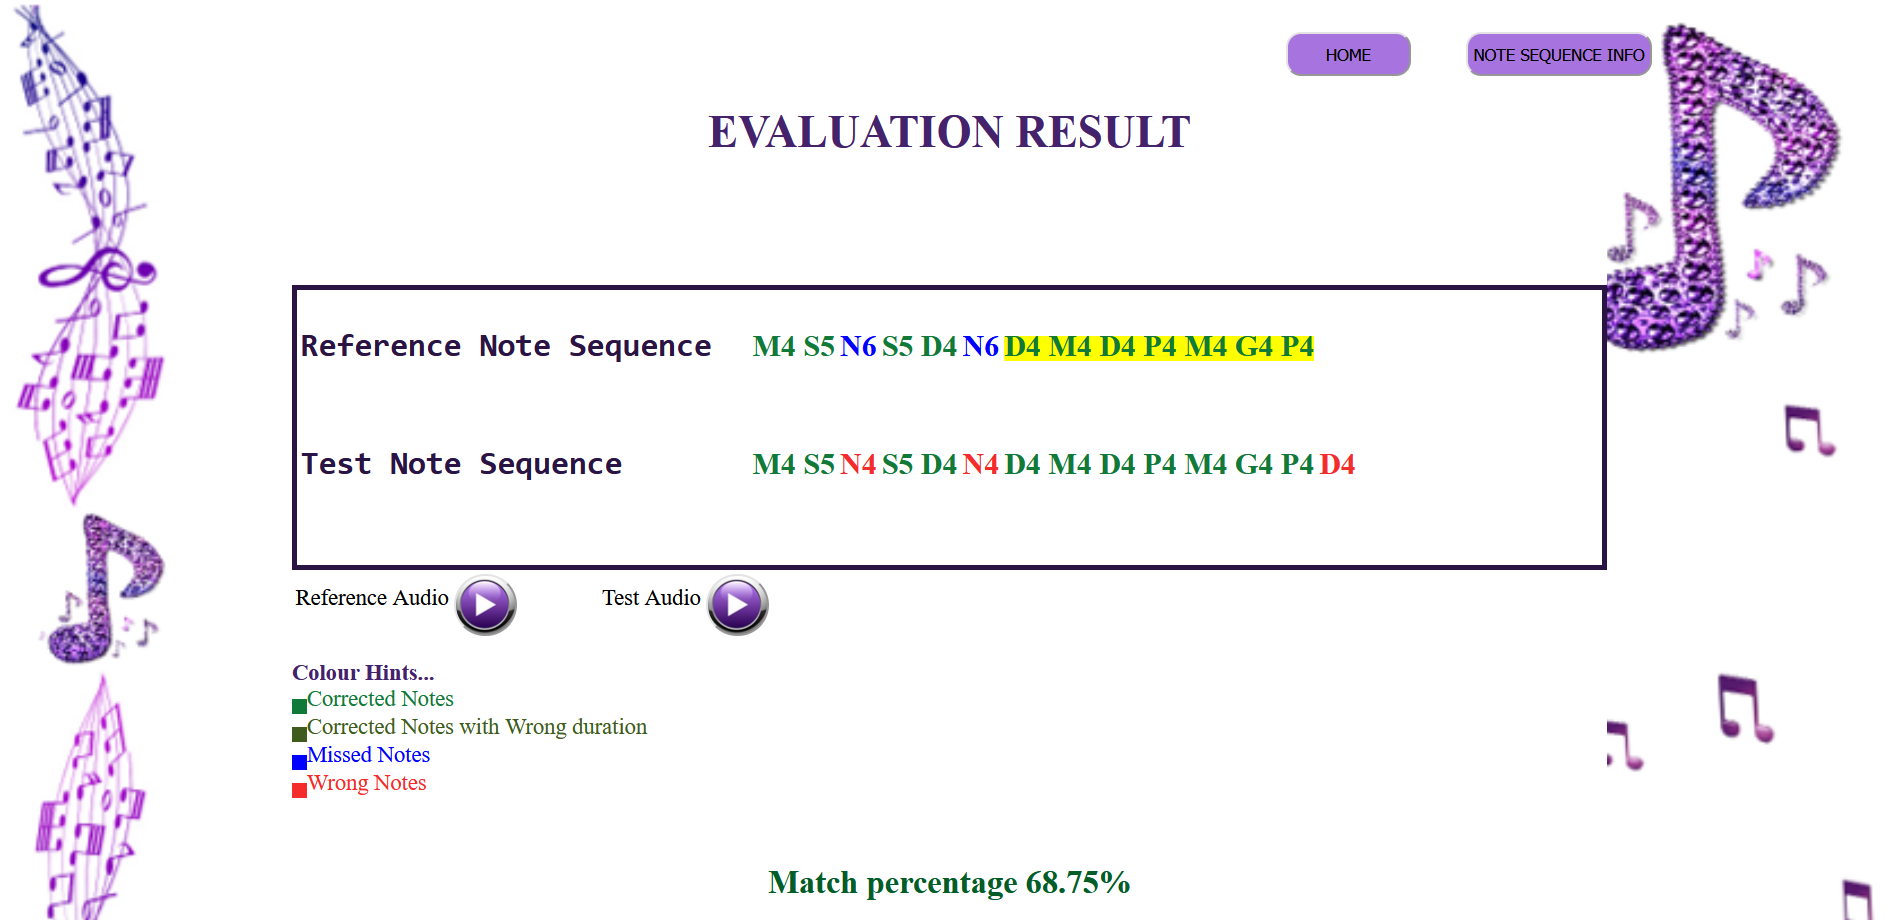
\includegraphics[scale=.27]{image/r11.png}}
% % 	\caption{Note sequence alignment of audio recordings}
% % 	\label{lvmh2}
% % \end{figure}
% % \FloatBarrier
% The following figure shows the time details of notes from audio inputs. 
% \vspace{1cm}
% \FloatBarrier
% \begin{figure}[h]
% 	\centering
% 	\fbox{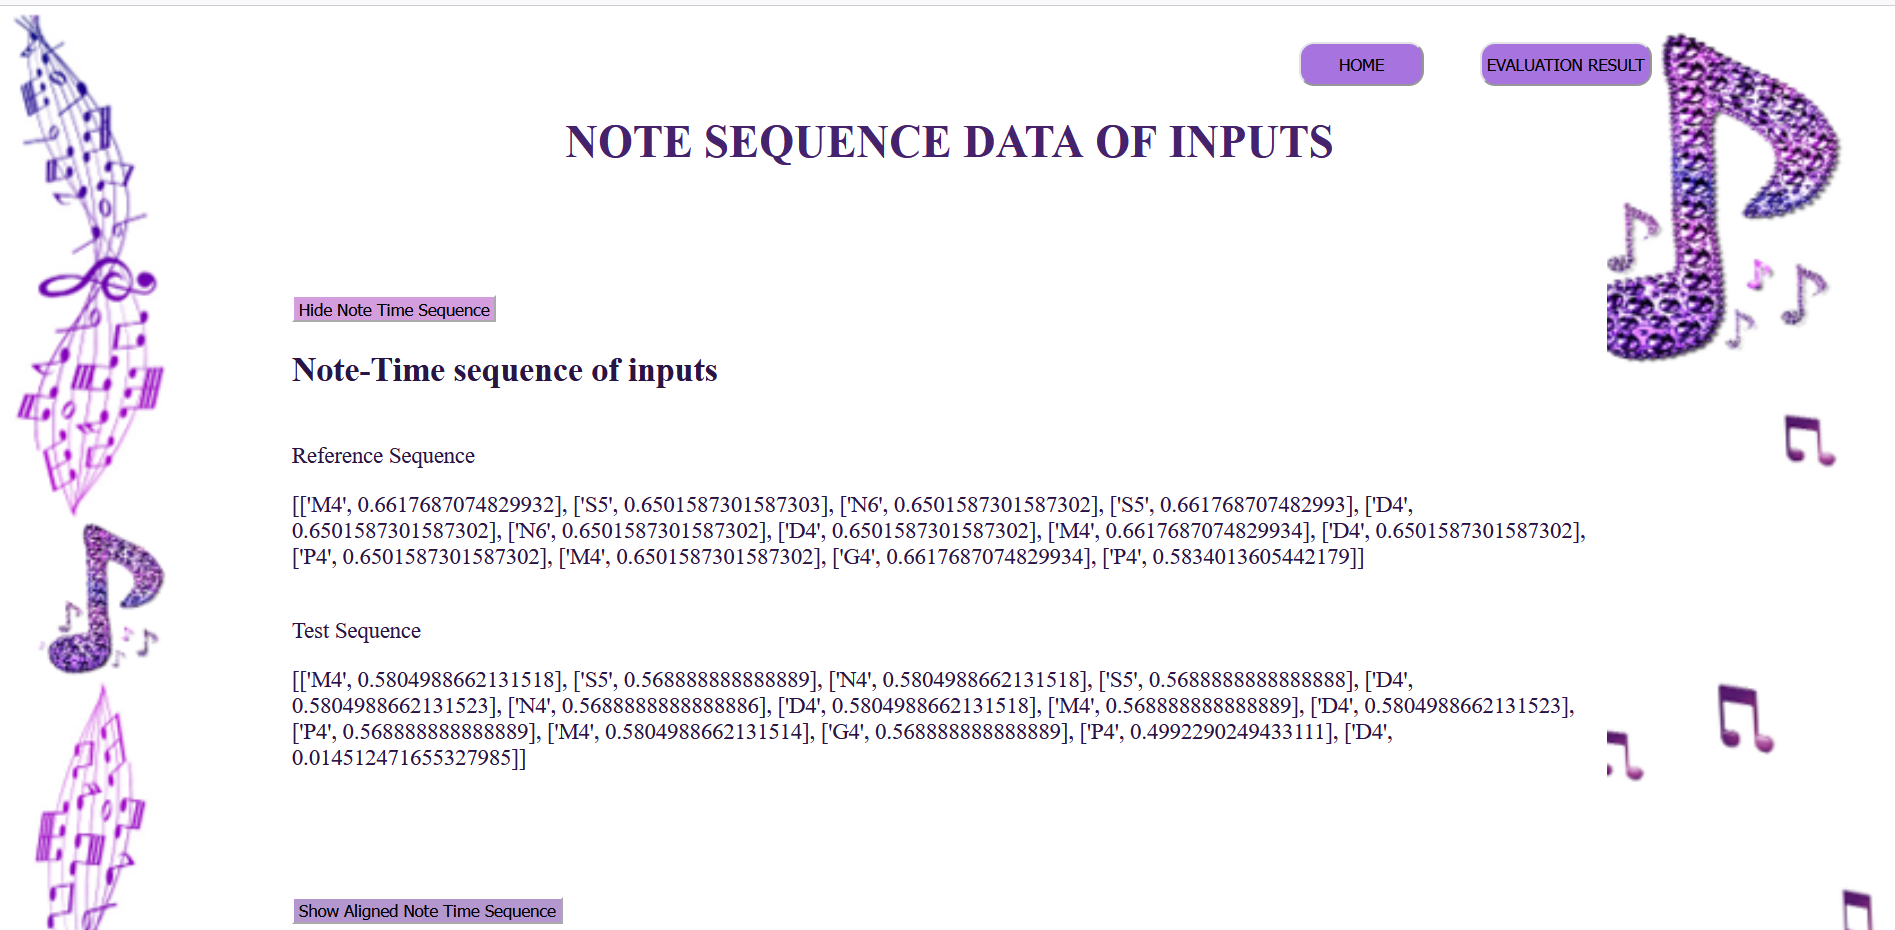
\includegraphics[scale=.27]{image/r12.png}}
% 	\caption{Display note time sequence}
% 	\label{lvmh2}
% \end{figure}
% \FloatBarrier
% The following figure shows the time duration details of notes and alignment between note sequences from audio inputs.
% \vspace{1cm}
% \FloatBarrier
% \begin{figure}[h]
% 	\centering
% 	\fbox{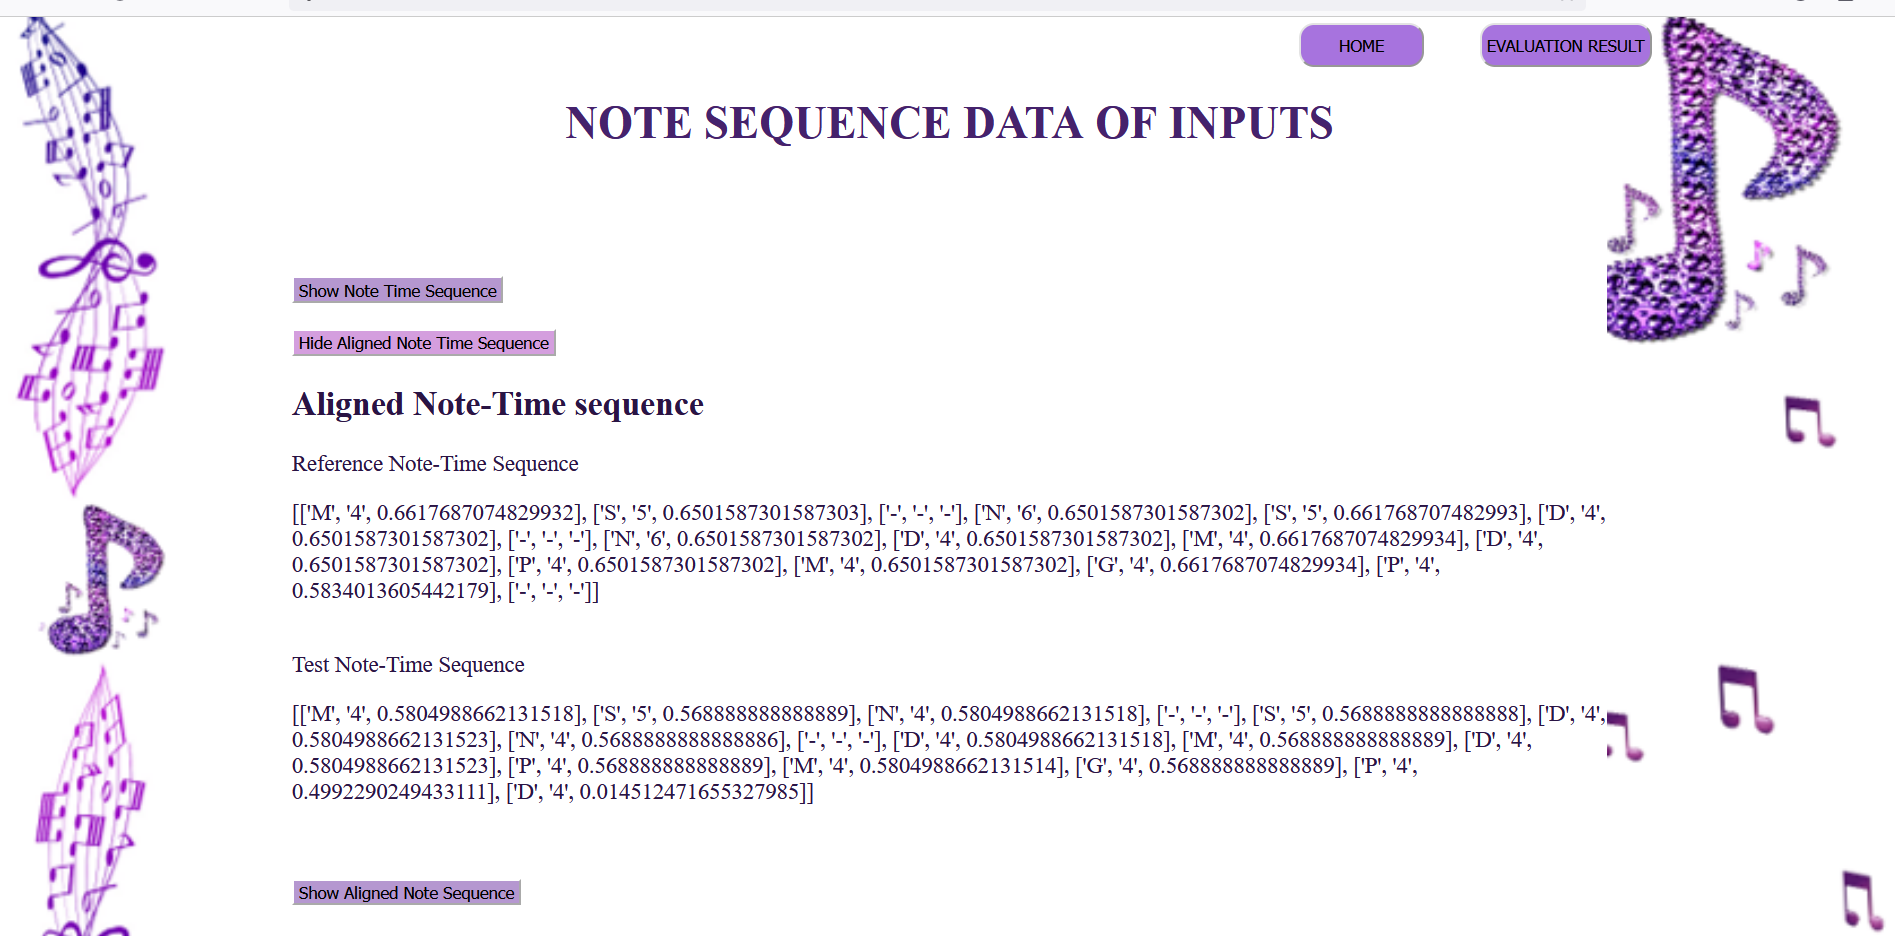
\includegraphics[scale=.27]{image/r13.png}}
% 	\caption{Display aligned note time sequence}
% 	\label{lvmh2}
% \end{figure}
% \FloatBarrier
% The following figure shows the alignment between note sequences by removing time duration from audio inputs.
%  \vspace{1cm}
% \FloatBarrier
% \begin{figure}[h]
% 	\centering
% 	\fbox{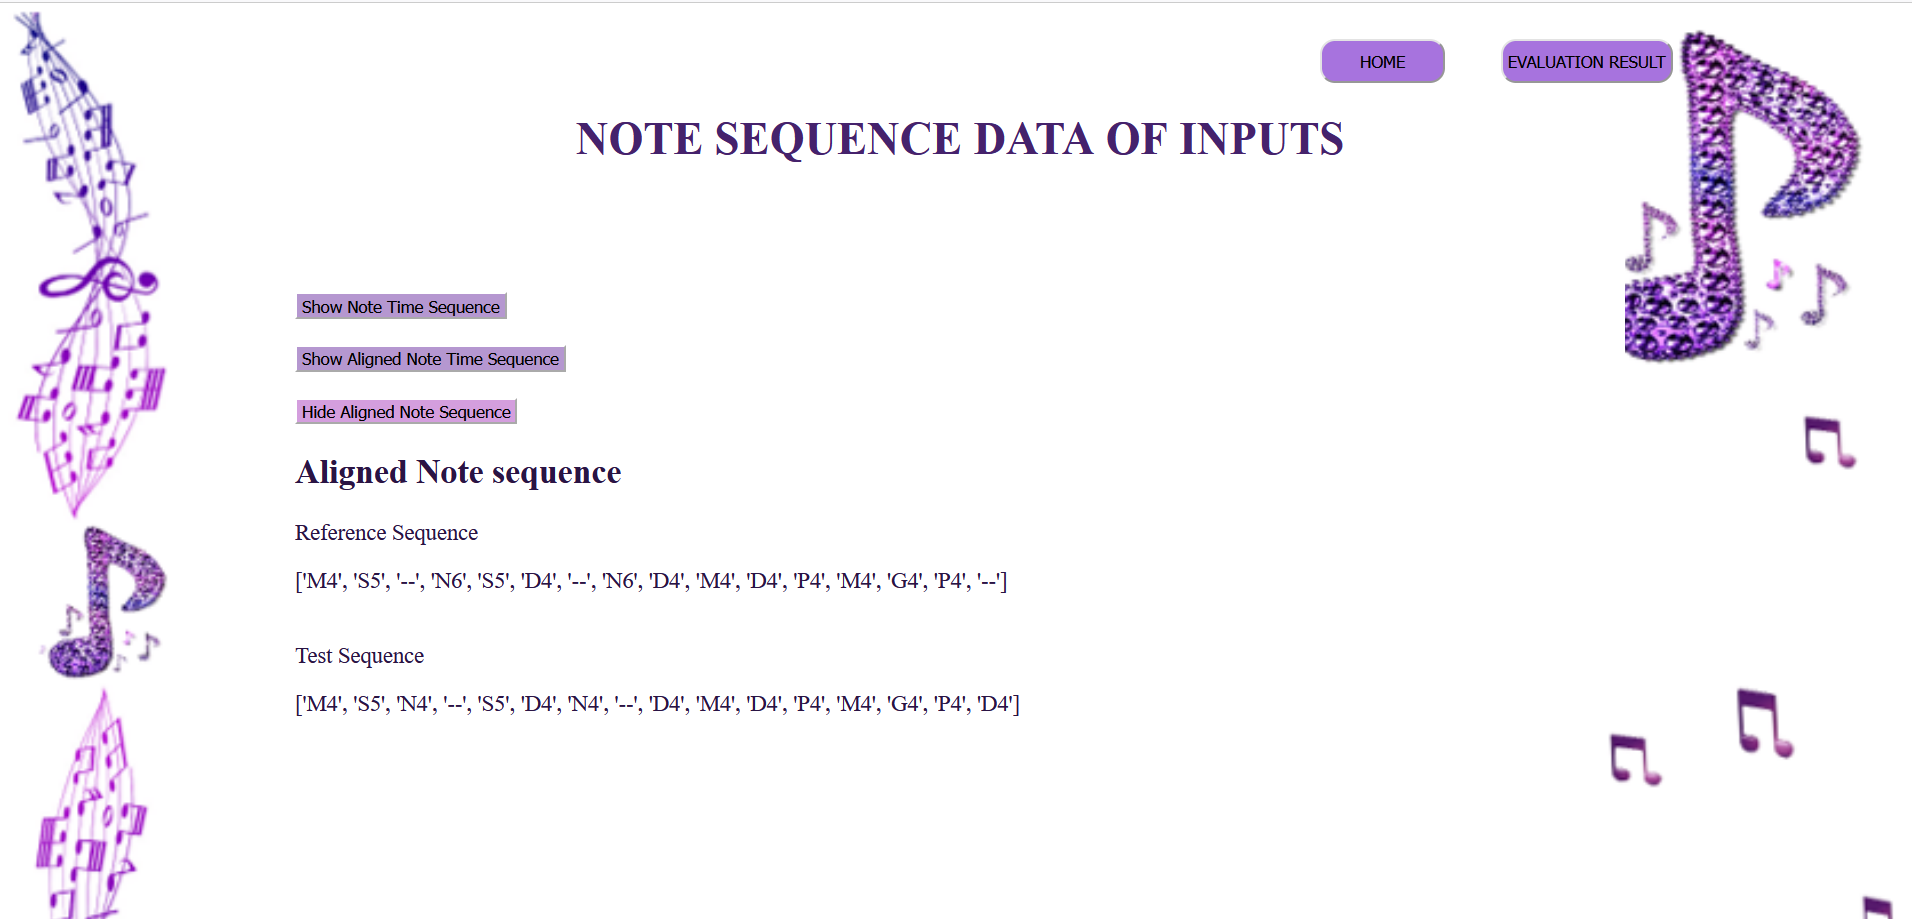
\includegraphics[scale=.27]{image/r14.png}}
% 	\caption{Display aligned note sequence}
% 	\label{lvmh2}
% \end{figure}
% \FloatBarrier
% \subsection{Accuracy in note sequence detection}
% The table below illustrates the accuracy of note sequence detection across various guitar audio recordings.
% \begin{table}[h]
%     \centering
%     \begin{tabular}{|c|c|c|c|}
%         \hline
%          \multirow{2}{*}{}  & Actual note & Detected note &   \\
%           & sequence & sequence & Match \\ 
%         % \thead{ } & \thead{Pitch, onset,\\ & and offset}  & \thead{Pitch and onset} & \thead{Onset only} & \thead{Offset only} \\
%         \hline
%         Guitar Audio 1 & M4 n4	D4	n4 P4 G4 & M4 n4	D4	n4 P4 G4 & \\
%         & D4	P4 M4	D4	M4 & D4	P4 M4	D4	M4 & 100\%\\
%         \hline
%          Guitar Audio 2 & M4 S5	N4	S5 D4   & M4 S5	N4	S5 D4 & \\
%         & N4 D4 M4 D4 P4 & N4 D4 M4 D4 P4 & \\
%          &  M4 G4 P4 & M4 G4 P4 & 100\%\\
%         \hline
%          Guitar Audio 3 & G4	 g4 G4 g4 m4    & G4	 g4 G4 g4 m4 & \\
%         & g4 m4 g4 m4 d4 & g4 m4 g4 m4 d4 & \\
%          &  D4 m4 g4  & D4 m4 g4 & 100\%\\
%         \hline
%          Guitar Audio 4 & d4 n4	D4	p4 P4 & d4 n4	D4	p4 P4 & \\
%         & g4	P4 M4 r4	M4 & g4	P4 M4 r4	M4 & 100\%\\
%         \hline
%          Guitar Audio 5 & s4 r4	G4	m4 P4  & s4 r4	G4	m4 P4 & \\
%           & m4 n4	G4	r4 G4  & m4 n4	G4	r4 G4 & \\
%         & D4 P4 M4	G4	r4 &  D4 P4 M4	G4	r4 & 100\%\\
%         \hline
%     \end{tabular}
%     \caption{Accuracy in detected note sequence of guitar music}
%     \label{tab:simple_table}
% \end{table}
% The table below illustrates the accuracy of note sequence detection across various piano audio recordings.
% \begin{table}[h]
%     \centering
%     \begin{tabular}{|c|c|c|c|}
%         \hline
%          \multirow{2}{*}{}  & Actual note & Detected note &   \\
%           & sequence & sequence & Match \\ 
%         % \thead{ } & \thead{Pitch, onset,\\ & and offset}  & \thead{Pitch and onset} & \thead{Onset only} & \thead{Offset only} \\
%         \hline
%         Guitar Audio 1 & M4 n4	D4	n4 P4 G4 & M4 n4	D4	n4 P4 G4 & \\
%         & D4	P4 M4	D4	M4 & D4	P4 M4	D4	M4 & 100\%\\
%         \hline
%          Guitar Audio 2 & M4 S5	N4	S5 D4   & M4 S5	N4	S5 D4 & \\
%         & N4 D4 M4 D4 P4 & N4 D4 M4 D4 P4 & \\
%          &  M4 G4 P4 & M4 G4 P4 & 100\%\\
%         \hline
%          Guitar Audio 3 & G4	 g4 G4 g4 m4    & G4	 g4 G4 g4 m4 & \\
%         & g4 m4 g4 m4 d4 & g4 m4 g4 m4 d4 & \\
%          &  D4 m4 g4  & D4 m4 g4 & 100\%\\
%         \hline
%          Guitar Audio 4 & d4 n4	D4	p4 P4 & d4 n4	D4	p4 P4 & \\
%         & g4	P4 M4 r4	M4 & g4	P4 M4 r4	M4 & 100\%\\
%         \hline
%          Guitar Audio 5 & s4 r4	G4	m4 P4  & s4 r4	G4	m4 P4 & \\
%           & m4 n4	G4	r4 G4  & m4 n4	G4	r4 G4 & \\
%         & D4 P4 M4	G4	r4 & D4 P4 M4	G4	r4 & 100\%\\
%         \hline
%     \end{tabular}
%     \caption{Accuracy in detected note sequence of piano music}
%     \label{tab:simple_table}
% \end{table}
%  To assess the accuracy of note sequences, several piano and guitar audio recordings were examined, revealing a 100\% accuracy rate. However, identifying the actual note sequence in vocal audio poses challenges due to variations in voice tone. But we can expect the note sequence of vocal audio. Here, the detected note sequence is also evaluated based on the expected note sequence. It provides accuracy of more than 80\% in vocal audio note sequence detection. If the audio is noise-free then it can provide 100\% accuracy. The proposed system can be used only for monophonic audio.
%  \subsection{ Result of Note sequence alignment}
%  The proposed Dynamic Time Warping algorithm has optimally aligned the note sequence, obtaining the maximum matching between note sequences. It accurately shows mistakes in test notes and provides a match score. Since the Dynamic Time Warping algorithm uses dynamic programming, its accuracy is 100\%.
% \par
% Figure 7.1 depicts the home page of the application. On the left side of the page, there are three buttons, while a frame is positioned on the right. The content within the frame dynamically changes according to the buttons clicked on the left side of the page. The first button name with \textbf{Create Tune} navigates to the tune creation process, the second button name with \textbf{Play Tune} leads to the tune playback process, and the third button name with \textbf{Convert to audio} directs to the audio conversion process.  
% \FloatBarrier
% \begin{figure}[h]
% 	\centering
% 	\fbox{\includegraphics[scale=.26]{image/result3.png}}
% 	\caption{Raga Selection}
% 	\label{lvmh2}
% \end{figure}
% \FloatBarrier

% Figure 7.2 shows the raga selection process initiated upon clicking the \textbf{Create Tune} button. It displays 72 raga options for selection. Upon choosing a raga, the interface navigates to another page, as represented in Figure 7.3. 



% \FloatBarrier
% \begin{figure}[h]
% 	\centering
% 	\fbox{\includegraphics[scale=.26]{image/result5.png}}
% 	\caption{Virtual Keyboard}
% \end{figure}
% \FloatBarrier

% \par Figure 7.3 demonstrates the presentation of a virtual keyboard corresponding to the selected raga. Each key on the virtual keyboard is associated with microtones of notes, concurrently mapped with the system keyboard labeled from 1 to 9. This interface enables the creation of note sequences. Additionally, this page offers options to customize instrument sounds, a button for tune replay, a slider to adjust speed, as well as buttons to save or discard tunes. When the 'Save' button is clicked, it prompts the user to enter a file name.

% \FloatBarrier
% \begin{figure}[h]
% 	\centering
% 	\fbox{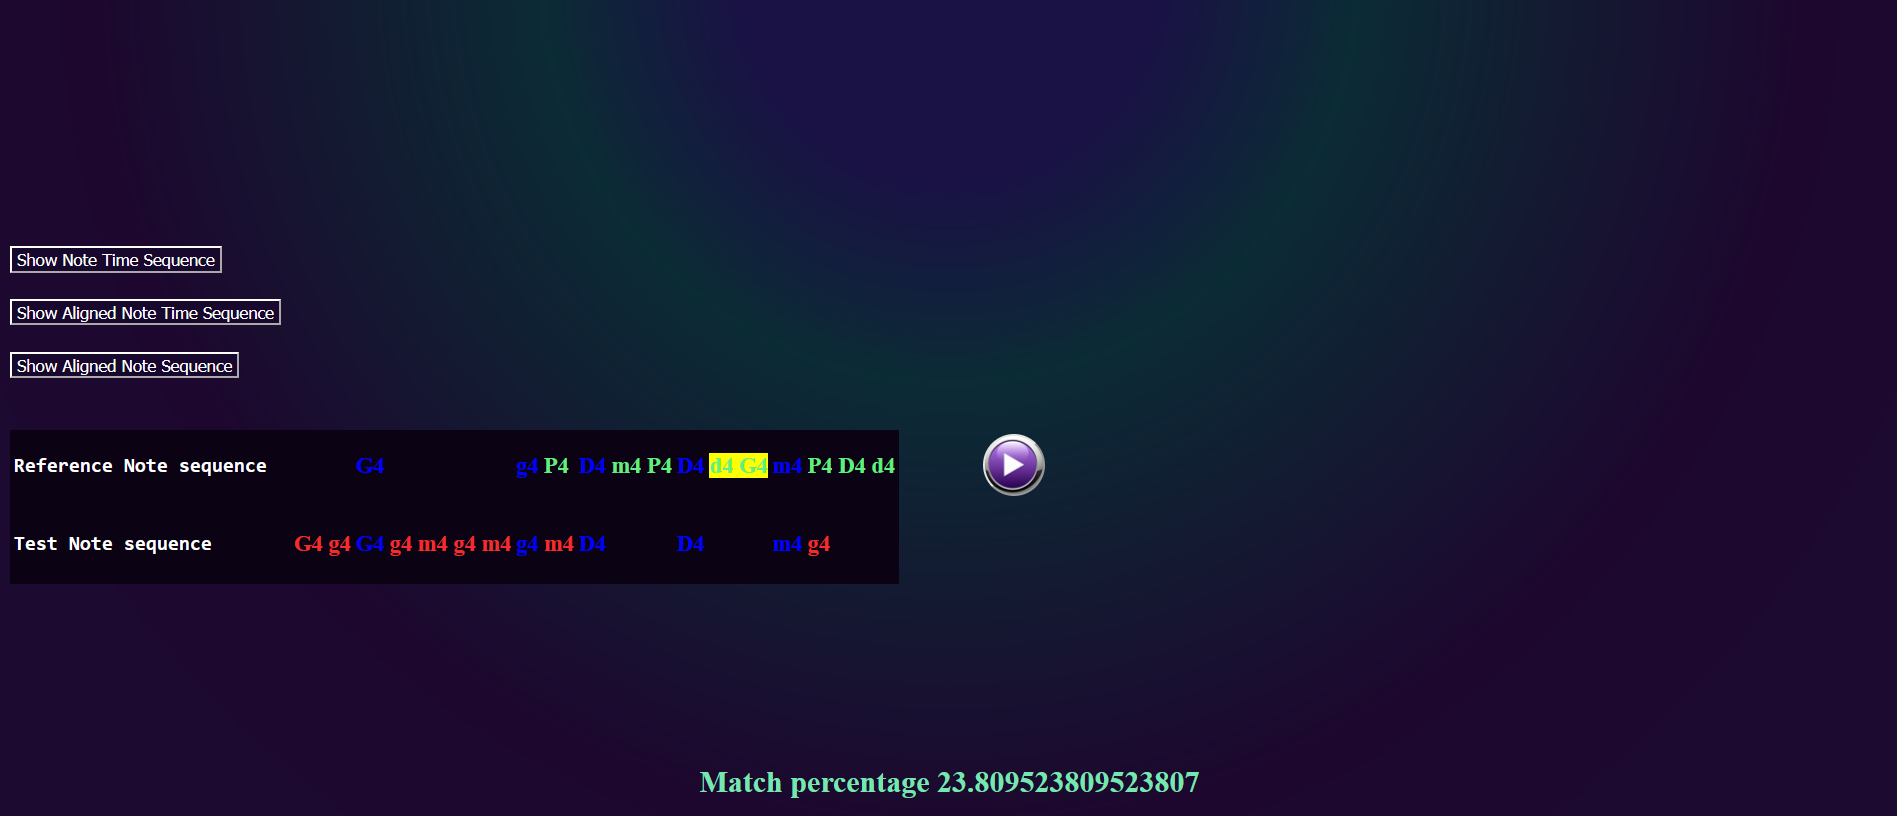
\includegraphics[scale=.26]{image/result7.png}}
% 	\caption{Playback Tune}
% \end{figure}
% \FloatBarrier

% \par Figure 7.4 demonstrates the tune-playing process initiated upon clicking the \textbf{Play Tune} button. This interface provides an input feature to upload a sequence file to play and offers options to customize instrument sounds, a button for tune play, and a slider to adjust speed.

% \FloatBarrier
% \begin{figure}[h]
% 	\centering
% 	\fbox{\includegraphics[scale=.26]{image/result9.png}}
% 	\caption{Input sequence file for audio conversion}
% \end{figure}
% \FloatBarrier
% % \par In figure 7.5, the same person's ECG is taken in a different date.

% % \FloatBarrier
% % \begin{figure}[h]
% % 	\centering
% % 	\fbox{\includegraphics[scale=.27]{image/result11.png}}
% % 	\caption{Sample Output 2}
% % \end{figure}
% % \FloatBarrier
% \par Figure 7.5 demonstrates the audio converting process initiated upon clicking the \textbf{Convert to Audio} button. This interface provides an input feature to upload a sequence file to convert into audio and offers options to customize instrument sounds, a button name with \textbf{Make Audio file}, and a slider to adjust speed. Upon clicking the \textbf{Make Audio file} button, the interface navigates to another page, as represented in Figure 7.6. 
% \FloatBarrier

% \begin{figure}[h]
% 	\centering
% 	\fbox{\includegraphics[scale=.26]{image/result10.png}}
% 	\caption{sequence file to audio conversion}
% \end{figure}
% \FloatBarrier
% \par Figure 7.6 illustrates the outcome after clicking the \textbf{Make Audio file} button. The  \textbf{Play} button enables previewing of the converted audio, and the  \textbf{Download} button allows users to download it. Upon clicking the \textbf{Download} button, the interface prompts the user to enter a file name, as represented in Figure 7.7. 

% \FloatBarrier
% \begin{figure}[h]
% 	\centering
% 	\fbox{\includegraphics[scale=.26]{image/result12.png}}
% 	\caption{Downloading audiofile}
% \end{figure}
% \FloatBarrier
% \textbf{Result:} All the functionalities provided in the system, such as raga selection, instrument selection, playback speed adjustment, playing tunes from sequence files, and audio conversion, are operating smoothly. The tune played from the sequence file achieves a 100\% accuracy rate. The audio obtained after converting the sequence file to an audio file precisely matches the played tune.

% \chapter{Evaluation and Results}

%\section{Performance Evaluation}
% \subsection{Evaluation Result}

% \subsubsection{Field Extraction Accuracy}
% Field extraction was carried out using a combination of libraries such as \texttt{pdfplumber} for digital PDFs and \texttt{pytesseract} with preprocessing techniques (binarization, noise removal, thresholding) for scanned images. The extracted text was cleaned and normalized using regular expressions and \texttt{numpy}.  

% For digital PDFs, the system extracted most fields accurately. Aadhaar numbers from Digilocker PDFs appeared masked (e.g., \texttt{XXXX XXXX 1234}), and Driving License numbers were extracted correctly but without spacing between the regional code and number (e.g., \texttt{KL089875678229} instead of \texttt{KL08 9875678229}). In rare cases (1 out of 8), the Aadhaar Name field concatenated with the address label due to formatting inconsistencies. Other fields such as Date of Birth, Gender, Address, SGPA, and Percentage were extracted with full accuracy.  

% When a scanned Aadhaar image (JPEG) was uploaded in addition to the PDFs, the full Aadhaar number was extracted successfully, and the Name concatenation issue was avoided, improving overall accuracy.  

% % \begin{table}[H]
% % \centering
% % \caption{Field-wise Accuracy (PDFs only)}
% % \begin{tabular}{|l|c|l|}
% % \hline
% % \textbf{Field} & \textbf{Accuracy} & \textbf{Remarks} \\ \hline
% % Name & 87--88\% & Correct in most cases. \\ \hline
% % Date of Birth & 100\% & Consistently extracted. \\ \hline
% % Gender & 100\% & Extracted from Aadhaar. \\ \hline
% % Aadhaar Number & 50\% & Masked in Digilocker PDFs  \\ \hline
% % PAN Number & 100\% & Fully extracted. \\ \hline
% % Driving License Number & $\sim$95\% & Value correct; spacing issue present. \\ \hline
% % Address & 100\% & Extracted reliably. \\ \hline
% % SGPA & 100\% & Extracted from marklists. \\ \hline
% % Percentage & 100\% & Extracted from marklists. \\ \hline
% % \end{tabular}
% % \end{table}

% \noindent Overall field extraction accuracy with only PDFs was approximately \textbf{88--90\%}, with main limitations being the masked Aadhaar number, minor formatting inconsistencies in Driving License numbers, and rare concatenation of Aadh-aar Name with Address.
% \subsection{Field Extraction Accuracy}
% \hspace{0.5cm} Field extraction used \texttt{pdfplumber} for digital PDFs and \texttt{pytesseract} with preprocessing (binarization, noise removal, thresholding) for scanned images. Text was cleaned and normalized with regular expressions and \texttt{numpy}.  

% Most fields were accurately extracted from PDFs. Aadhaar numbers from Digilocker PDFs were masked (e.g., \texttt{XXXX XXXX 1234}) and Driving License numbers lacked spacing (e.g., \texttt{KL089875678229}). Rarely, the Aadhaar Name concatenated with the address. Other fields, including Date of Birth, Gender, Address, SGPA, and Percentage, were fully extracted.  

% Adding scanned Aadhaar images resolved masking and concatenation issues. Overall field extraction accuracy with PDFs alone was around \textbf{88--90\%}, with minor limitations due to masked Aadhaar numbers and formatting inconsistencies.



% \subsection{Consolidated Profile Accuracy}
% \hspace{0.3cm} The consolidation step merged extracted fields from multiple documents into a unified profile. Conflicts (e.g., different spellings of a name or minor formatting differences) were resolved using frequency-based selection and semantic similarity matching with \texttt{sentence-transformers}.  
% Across all tested cases, the system achieved \textbf{100\% consolidation accuracy}, producing reliable profiles.

% \subsection{Form Auto-Filling Accuracy}
% \hspace{0.3cm} For form filling, extracted fields were mapped to target form fields using semantic similarity techniques. Even when labels in the form were phrased differently (e.g., ``DOB'' vs ``Date of Birth''), the model correctly identified matches. The auto-fill module then populated the fields using Python browser automation.  
% In testing with 16 expected form fields, the system filled all fields correctly, resulting in a \textbf{100\% form filling accuracy}.

% \subsection{User Verification and Correction Rate}
% \hspace{0.3cm} Once the form was auto-filled, users could review the results. Since the system’s accuracy was very high, manual corrections were rarely required. For digital PDFs alone, Aadhaar numbers required correction due to masking, and the occasional Name concatenation had to be fixed. With supporting Aadhaar images provided, no manual corrections were necessary, except for minor adjustments in the Driving License number formatting.  
% This gives the system an effective correction rate of \textbf{0--2\%}, showing strong reliability.

% \subsubsection{Processing Time}
% The system processed digital PDFs efficiently, completing extraction and form filling in an average of \textbf{3--5 seconds} for four documents. When scanned images were included, the time increased slightly due to OCR preprocessing, averaging \textbf{5--7 seconds}, which is still acceptable for practical use. 
% \subsection{Processing Time}
% \hspace{0.3cm} The system processed digital PDFs efficiently, completing extraction and form filling in an average of \textbf{3--5 seconds} for four documents. When scanned images were included, the time increased slightly due to OCR preprocessing, averaging \textbf{5--7 seconds}. These times were measured by recording the duration from the moment documents were uploaded to the point when the form was fully autofilled, using Python's built-in timing functions, which provides a practical estimate of real-world performance.

% \newpage
% \subsection{Observations}
% \begin{itemize}
%     \item Digital PDFs achieved high accuracy, but Aadhaar numbers were masked in Digilocker files.
%     \item In 1 of 8 cases, the Aadhaar Name field concatenated with the Address, slightly reducing accuracy.
%     \item Adding scanned Aadhaar images resolved masking and name concat-enation, improving accuracy to nearly 100\%.
%     \item Driving License numbers were correct but spacing inconsistencies slightly reduced accuracy.
%     \item The auto-filling module demonstrated robustness by correctly mapping fields even with inconsistent naming.
%     \item Minimal user corrections were required, confirming the system’s efficie-ncy and practicality.
% \end{itemize}

% \subsection*{\hspace{-0.1cm}Observations}
% \begin{itemize}
%     \item Digital PDFs were generally accurate, though Aadhaar numbers were masked.
%     \item Rarely, Aadhaar Name concatenated with the Address, slightly reducing accuracy.
%     \item Adding scanned Aadhaar images resolved masking and concatenation issues.
%     \item Driving License numbers had minor spacing inconsistencies.
%     \item Auto-filling correctly mapped fields even with inconsistent naming.
%     \item Minimal user corrections were needed, confirming system reliability.
% \end{itemize}

\chapter{CONCLUSION}

\hspace{0.5cm} The proposed AI-Powered Code Document Generator would thus offer an intelligent and automated solution for the generation of accurate, structured, and context-aware documentation from source code. This would thus help in the identification of significant software components like functions, classes, imports, call relationships, entry points, and recursive patterns, among others. In this regard, the proposed solution would leverage Tree-sitter for parsing code across fourteen programming languages and thus generate accurate documentation like the README file, architecture, description of files, recent changes of the git repository, among others.

\par The system relies on a three-stage feature extraction process to guarantee the LLM access to rich and non-redundant information for every function it documents. Features extracted from the AST offer structural information such as the function’s name, class membership, parameters, return type, and calls. Features extracted from the text offer context-based information on the file’s complexity and documentation. Features extracted from the graph offer architectural information on the function and the program based on the NetworkX library’s directed call graph. By combining all the features in a single fact block, the system offers documentation that is functionally correct, contextually scaled and architecturally aware.

\par This modular and language-independent design ensures that each module is independent in its functioning through well-defined interfaces. It is possible to upgrade or extend any module in the pipeline without affecting the rest of the pipeline. Cross-file awareness ensures that functions used across module boundaries are correctly identified as active rather than unused, thereby improving the reliability of the architectural analysis. The parallel document generation using the \texttt{ThreadPoolExecutor} ensures the pipeline scales well with projects of different sizes.

\par This tool is highly beneficial for software development teams working with repositories that lack adequate documentation. It boosts productivity by automating what is usually a manual and time-consuming process. Additionally, it supports long-term code maintainability by allowing developers to understand the code’s structure through graph-based analysis.

\par Overall, the project highlights the potential of combining artificial intelligence with static code analysis to create a practical tool that simplifies software documentation. Future improvements could include extending support to more programming languages, integrating with version control systems to enable real-time documentation updates and employing more advanced language models for richer, more detailed explanations, ultimately developing the system into a comprehensive, production-ready documentation platform.
\newline
\par Despite the current system addressing many key challenges in automated documentation, there is room for improvement by enhancing system capabilities, supporting additional programming languages and adding new features to make the system more intelligent and adaptive. These opportunities pave the way for future developments that could increase the system’s effectiveness and applicability in real-world software development scenarios which discussed in next chapter.
\chapter{FUTURE ENHANCEMENT}

\hspace{0.5cm} The AI-Powered Code Document Generator sets a robust foundation for automated documentation, demonstrating how static code analysis and large language models can work together to produce accurate, structured and context-rich documentation for multiple programming languages. This chapter explores several opportunities for enhancing and refining the system to advance it toward a more comprehensive, production-ready platform.

\section{Git Integration}
\hspace{0.5cm} One of the way to improve the system would be to integrate it more closely with Git-based platforms like GitHub and GitLab. Currently, documentation is generated when a user provides a repository URL or manually uploads files. Enhanced Git integration could allow the documentation to update automatically with each commit.



\section{Multi-Language Expansion}
\hspace{0.5cm} Although the system currently supports fourteen programming languages, future upgrades could add support for languages like Swift, Scala, Dart and Haskell. Expanding language compatibility would make the system applicable to a wider range of development projects beyond its current scope.


\section{Interactive Q\&A}
\hspace{0.5cm} A highly valuable future feature could be the addition of an intelligent Question\&Answer system (Q\&A ), allowing developers to interact with the codebase through a natural language interface. Instead of merely reviewing the automatically generated documentation, developers could directly ask questions about function call chains, recent changes or other specific aspects of the system.



\hspace{0.5cm}The future improvements proposed in this chapter represent a natural progression of the current system. Git integration would embed documentation generation into the ongoing development workflow. Expanding multi-language support would broaden the system’s applicability across diverse programming environments. Adding an interactive Q\&A feature would transform the system from a passive documentation generator into an active tool for code understanding. Collectively, these enhancements would result in a highly efficient and practical automated documentation platform.
%\input{tex/bibliography}
%\setcounter{chapter}{0}

\renewcommand{\chaptername}{annexure}

%\pagenumbering{arabic}
%{\renewcommand{\addtocontents}[2]{}
\addcontentsline{toc}{chapter}{Annexure 1}
\addtocontents{toc}{\protect\setcounter{tocdepth}{-1}}
\chapter{Algorithms and Flow Charts}
\section{LZW encoding}

\begin{algorithm}[H]
 \KwIn{String $\omega$}
 \KwOut{Compressed codewords}
 \Begin{
 \textbf{Step:}Read next input character K
 \eIf{no such K (input exhausted)}{
 	code($\alpha$)$\rightarrow$ output;
 	EXIT;
 }{
 	\eIf{$\alpha$K exists in string table}{
 		$\alpha$K$\rightarrow \alpha$;
 		Repeat \textbf{Step};
 	}{
 		code($\alpha$)$\rightarrow$ output;
 		$\alpha$K$\rightarrow$ string table;
 		K $\rightarrow \alpha$;
 		Repeat \textbf{Step};
 	}
 }
 }
 \caption{LZW encoding}
 \label{lzwAlgo}
 \end{algorithm}
\newpage
\section{Data De-duplication}

\begin{algorithm}
 \KwIn{Data segment}
 \KwOut{Index, deduplicated data segment}
 \Begin{
 Initialize: $p = false,\ size = 1,\ inc = \Delta d,\ blockPointer = 0,\ buffer = \phi$ \;
 \textbf{A:} Retrieve block at $blockPointer$, append retrieved block to buffer\;
 Calculate hash of the buffer\;
 \eIf{hash is in dictionary}{
 	set: $p=true$\;
 	$size+=1$ \;
 	$blockPointer += inc*x$\;
 	$\Delta d = blockSize/x$\;
 	\eIf{End of segment}{
 		Goto \textbf{D}\;
 	}{
 		Goto \textbf{A}\;
 	}
 }{
 	Insert hash into dictionary\;
 	\eIf{$p=false$}{
 		$blockPointer += inc * x$\;
 		Goto \textbf{B}\;
 	}{
 		Generate index for previous non-unique block\;
 		$blockPointer += inc * x$, $p=false$, $size = 0$, $buffer=\phi$\;
 		\textbf{C:} \eIf{End of Segment}{
 			Goto \textbf{E}\;
 		}{
 			Goto \textbf{A}\;
 		}
 	}
 }
 
 \textbf{B:} Set $nextBlockPointer = blockPointer + (inc*x)$\;
 increment $blockPointer$ by $inc$\;
 set $prevBuffer = buffer$\;
 clear $buffer$\;
 }
 \caption{De-duplication algorithm.}
 \label{deDupAlgo1}
\end{algorithm}
\newpage
	\begin{algorithm}[]
 \KwIn{Index, deduplicated data segment}
 \KwOut{Original data}
 \Begin{
 \textbf{F:} Retrieve block at $blockPointer$\;
 Calculate hash\;
 \eIf{hash in dictionary}{
 	Output non-duplicate data between blocks, generate index\;
 	Goto \textbf{A}\;
 }{
 	Increment $blockPointer$ by $inc$\;
 	Clear buffer\;
 	\eIf{$blockPointer = nextBlockPointer$}{
 		decrement $blockPointer$ by $(inc*x)$\;
 		retrieve block at $blockPointer$ and append to $prevBuffer$\;
 		Calculate hash and add to dictionary\;
 		Goto \textbf{C}\;
 	}{
 		Goto \textbf{F}\;
 	}
 }
 \textbf{D:} Generate Index\;
 \textbf{E:} End\;
 
 Read the first/next block\;
 Check index for the current read offset\;
 \eIf{data block}{
 		Output the block as it is\;
 	}{
 		Obtain starting memory offset from the index\;
 		Duplicate the data from starting memory offset for the specified number of blocks\;
 	}
 \If{Last block}{
 	Exit;
 }
  }
 \caption{De-duplication algorithm (cont).}
 \label{deDupAlgo2}
\end{algorithm}
\newpage
\section{Delta Encoding}
\begin{algorithm}[H]
 \KwIn{De-duplicated data}
 \KwOut{Delta Graph}
 \Begin{
 \textbf{set} blocks = segment\_size / 50000\;
 \textbf{set} i = 0\;
 \While{i $<$ blocks}{
 	\textbf{set} node[i].sim = 0\;
 	\textbf{set} node[i].ref\_block = -1\;
 	\textbf{set} node[i].data = dataBlock[i]\;
 	\textbf{set} node[i].fuzzy\_hash = fuzzy hash of data\;
 	\textbf{set} node[i].node\_size = node[i].data.size\;
 	\textbf{increment} i\;
 }
 \textbf{set} i = 0 \;
 \While{i $<$ blocks}{
 	\textbf{set} j = i + 1\;
 	\While{j $<$ blocks}{
 		\textbf{set} similarity = fuzzy\_compare(node[i].fuzzy\_hash, node[j].fuzzy\_hash)\;
 		\If{similarity $>$ threshold \textbf{and} node[j].sim $<$ similarity}{
 			\textbf{set} node[j].sim = similarity\;
 			\textbf{set} node[j].ref\_node = i\;
 		}
 		\textbf{increment} j\;
 	}
 	\textbf{increment} i\;
 }	
 
 }
 
 
 \caption{Delta Graph Generation}
 \label{cgAlgo}
 \end{algorithm}
 
\begin{algorithm}[H]
 \KwIn{Delta Graph}
 \KwOut{Delta Encoded Nodes}
 \Begin{
 \textbf{set} blocks = segment\_size / 50000\;
 \textbf{set} i = 0\;
 \textbf{set} threshold = 10\;
 \While{i $<$ blocks}{
 	\If{node[i].ref\_node $\neq$ -1}{
 		\textbf{set} node[i].data = deltaEncode(node[i], node[i].ref\_node)\;
 		\textbf{set} node[i].node\_size = node[i].data.size\;
 	}
 	
 	\textbf{set} outData = concatenate (node[i].node\_size, node[i].ref\_node, node[i].data)\;
 	\textbf{output} outData\;
 	\textbf{incerment} i\;
 }
 
 }
 
 
 \caption{Delta Encoding}
 \label{delAlgo}
 \end{algorithm}
\newpage
\section{Flow Charts}
\begin{figure}[th]
	\centering
	\includegraphics[scale=0.5]{deDup1}
	\caption{De duplication Algorithm}
	\label{lvmh1}
\end{figure}
\newpage
\begin{figure}
	\centering
	\includegraphics[scale=0.6]{deDup2}
	\caption{De duplication Algorithm (cont.)}
	\label{lvmh2}
\end{figure}

 \addtocontents{toc}{\protect\setcounter{tocdepth}{5}}


\newpage
\begin{thebibliography}{10}

\bibitem{Song2024}
J. Song, Z. Zhang, Z. Tang, S. Feng, and Y. Gu,
``Improving Code Summarization With Tree Transformer Enhanced by Position-Related Syntax Complement,''
\emph{IEEE Transactions on Artificial Intelligence}, vol. 5, no. 9, pp. 4776--478X, Sept. 2024, doi: 10.1109/TAI.2024.3395231.
\bibitem{Rozi2023}
M. F. Rozi, T. Ban, S. Ozawa, A. Yamada, T. Takahashi, S. Kim, and D. Inoue,
``Detecting Malicious JavaScript Using Structure-Based Analysis of Graph Representation,''
\emph{IEEE Access}, vol. 11, pp. 102727--1027XX, 2023, doi: 10.1109/ACCESS.2023.3317266.

\bibitem{Mostafavi2024}
M. M. Ghahfarokhi, A. Khademian, S. Kianiangolafshani, A. Asadi, H. Jahantigh, and A. Heydarnoori,
``Beyond Syntax: Unleashing the Power of Computational Notebooks Code Metrics in Documentation Generation,''
in \emph{Proc. IEEE/ACM Int. Conf. AI Engineering -- Software Engineering for AI (CAIN)}, Lisbon, Portugal, Apr. 2024, pp. 278--280, doi: 10.1145/3644815.3644979.

\bibitem{Wang2020}
W. Wang, Y. Zhang, Y. Sui, Y. Wan, Z. Zhao, J. Wu, P. S. Yu, and G. Xu,
``Reinforcement-Learning-Guided Source Code Summarization using Hierarchical Attention,''
\emph{IEEE Transactions on Software Engineering}, 2020.
\bibitem{CodeDocAgent2025}
S. Yao, Y. Shen, D. Liu, and J. Hu,
``CodeDocAgent: Leveraging Large Language Models for Accurate and Contextual Code Documentation,''
in \emph{Proceedings of IEEE}, 2025.

\bibitem{Zhu2025}
Y. Zhu, X. Zhao, X. Li, Y. Zou, H. Yuan, Y. Wang, and B. Xie,
``RepoSummary: Feature-Oriented Summarization and Documentation Generation for Code Repositories,''
in \emph{Proc. ACM Conf.}, 2025.

\bibitem{KhanUddin2023}
J. Y. Khan and G. Uddin,
``Combining Contexts from Multiple Sources for Documentation-Specific Code Example Generation,''
in \emph{Proc. IEEE Int. Conf. Software Analysis, Evolution and Reengineering (SANER)}, 2023, pp. 683--693, doi: 10.1109/SANER56733.2023.00071.

\bibitem{Thota2024}
S. R. Thota, S. Arora, and S. Gupta,
``AI-Driven Automated Software Documentation Generation for Enhanced Development Productivity,''
in \emph{Proc. Int. Conf. Data Science and Network Security (ICDSNS)}, 2024.

\bibitem{GhaleDabbagh2025}
D. P. Ghale and M. Dabbagh,
``Automated Code Comments Generation Using Large Language Models: Empirical Evaluation of T5 and BART,''
\emph{IEEE Access}, vol. 13, pp. 141420--1414XX, 2025, doi: 10.1109/ACCESS.2025.3597601.










\bibitem{Procko2023}
T. T. Procko and S. Collins, ``Automatic Code Documentation with Syntax Trees and GPT: Alleviating Software Development’s Most Redundant Task,'' Embry-Riddle Aeronautical University, Daytona Beach, FL, USA.

\end{thebibliography}

\addcontentsline{toc}{chapter}{Bibliography}
% \bibliographystyle{unsrt}
% %\pagestyle{plain}
% \bibliography{bib/thesis}





















\end{spacing}








\end{document}
